% Gabarit pandoc des corrigés publiés (brut et guidé). Contenu sans marque ni nom de site.
% Compilation : lualatex (latexmk -lualatex).
% Le Markdown reste la source unique : ne pas éditer ce fichier .tex à la main.
\documentclass[11pt,a4paper]{article}

% --- Moteur, polices (Latin Modern) et langue ---------------------------------
\usepackage{iftex}
\ifLuaTeX\else\errmessage{Ce document se compile avec lualatex}\fi
\usepackage{amsmath,amssymb,mathtools}
\usepackage{fontspec}
% mathrm=sym : \mathrm prend ses glyphes dans la police mathématique (ℓ, μ, Ω), comme KaTeX.
\usepackage[math-style=TeX,bold-style=TeX,mathrm=sym]{unicode-math}
% Repli pour les glyphes absents de Latin Modern (indices et exposants Unicode,
% flèches, filets des schémas en texte, symboles) : DejaVu, puis Latin Modern Math
% (ℓ, lettres mathématiques Unicode des légendes).
\directlua{
  luaotfload.add_fallback("repliTexte", {"DejaVuSerif:mode=harf;", "DejaVuSans:mode=harf;", "file:latinmodern-math.otf:mode=harf;"})
  luaotfload.add_fallback("repliMono", {"DejaVuSansMono:mode=harf;", "DejaVuSans:mode=harf;", "file:latinmodern-math.otf:mode=harf;"})
}
\setmainfont{Latin Modern Roman}[RawFeature={fallback=repliTexte}]
\setsansfont{Latin Modern Sans}[RawFeature={fallback=repliTexte}]
\setmonofont{Latin Modern Mono}[RawFeature={fallback=repliMono}]
\setmathfont{Latin Modern Math}
\usepackage[french]{babel}
\frenchsetup{SmallCapsFigTabCaptions=false}

% --- Mise en page --------------------------------------------------------------
\usepackage[a4paper,margin=2.2cm,headheight=14pt,footskip=1.2cm]{geometry}
\usepackage{microtype}
\setlength{\emergencystretch}{4em}
\tolerance=1500
\setlength{\parindent}{0pt}
\setlength{\parskip}{0.55\baselineskip plus 2pt minus 1pt}
\usepackage{xcolor}
% Gris nommés : babel-french rend « ! » actif dans le document.
\definecolor{gris2}{gray}{0.98}
\definecolor{gris3}{gray}{0.97}
\definecolor{gris5}{gray}{0.95}
\definecolor{gris35}{gray}{0.65}
\definecolor{gris40}{gray}{0.60}
\definecolor{gris45}{gray}{0.55}
\definecolor{gris50}{gray}{0.50}
\definecolor{gris55}{gray}{0.45}
\definecolor{gris60}{gray}{0.40}
\definecolor{gris65}{gray}{0.35}
\definecolor{gris70}{gray}{0.30}
\definecolor{gris80}{gray}{0.20}
\definecolor{gris85}{gray}{0.15}
\usepackage{graphicx}
\usepackage{float}
\usepackage{caption}
\captionsetup{font=small,labelformat=empty,justification=centering}
\usepackage{booktabs,longtable,array,multirow,calc}
\usepackage{siunitx}
\sisetup{locale=FR}
\usepackage[version=4]{mhchem}
\usepackage{listings}
\usepackage{fancyhdr}
\usepackage{lastpage}
\usepackage[most]{tcolorbox}
\usepackage{enumitem}
\setlist{nosep,leftmargin=*,topsep=2pt}
\usepackage[hidelinks,unicode]{hyperref}
\usepackage{bookmark}
\hypersetup{pdftitle={Banque PT PT — Sciences industrielles C 2026},pdfauthor={Rédigé par IA},pdfcreator={LaTeX},pdfsubject={Corrigé guidé}}
\usepackage{xurl}

% --- Pandoc : listes, tableaux, figures ----------------------------------------
\providecommand{\passthrough}[1]{#1}
\providecommand{\tightlist}{\setlength{\itemsep}{0pt}\setlength{\parskip}{0pt}}

\makeatletter
\def\maxwidth{\ifdim\Gin@nat@width>\linewidth\linewidth\else\Gin@nat@width\fi}
\def\maxheight{\ifdim\Gin@nat@height>0.55\textheight 0.55\textheight\else\Gin@nat@height\fi}
\makeatother
\setkeys{Gin}{width=\maxwidth,height=\maxheight,keepaspectratio}
\setcounter{secnumdepth}{-\maxdimen}
\providecommand{\pandocbounded}[1]{#1}
\usepackage{longtable,booktabs,array}

% --- Code (listings) -----------------------------------------------------------
\lstset{
  basicstyle=\ttfamily\small,
  columns=fullflexible,
  keepspaces=true,
  breaklines=true,
  breakatwhitespace=false,
  postbreak=\mbox{\textcolor{gris50}{$\hookrightarrow$}\space},
  frame=single,
  rulecolor=\color{gris35},
  framesep=4pt,
  xleftmargin=5pt,xrightmargin=5pt,
  backgroundcolor=\color{gris3},
  keywordstyle=\bfseries,
  commentstyle=\color{gris65},
  stringstyle=\color{gris80},
  showstringspaces=false,
  tabsize=4,
  extendedchars=true,
  aboveskip=6pt,belowskip=6pt,
}

% --- Macros des corrigés (KaTeX ↔ LaTeX) ---------------------------------------
% Les corrigés sont écrits pour KaTeX : on définit ici ce que KaTeX connaît et
% que LaTeX n'a pas, sans jamais retoucher le Markdown.
\providecommand{\R}{\mathbb{R}}
\providecommand{\N}{\mathbb{N}}
\providecommand{\Z}{\mathbb{Z}}
\providecommand{\Q}{\mathbb{Q}}
\providecommand{\C}{\mathbb{C}}
\providecommand{\dd}{\mathrm{d}}
\providecommand{\llbracket}{\lBrack}
\providecommand{\rrbracket}{\rBrack}
\providecommand{\lBrace}{\lbrace}
\providecommand{\rBrace}{\rbrace}
\providecommand{\Box}{\square}
\providecommand{\Diamond}{\lozenge}
\providecommand{\varnothing}{\emptyset}
\providecommand{\argmax}{\operatorname*{arg\,max}}
\providecommand{\argmin}{\operatorname*{arg\,min}}
\renewcommand{\leq}{\leqslant}
\renewcommand{\geq}{\geqslant}

% Équation hors texte : réduite à la largeur de la ligne si elle déborde.
\newsavebox{\boiteequation}
\newcommand{\equationajustee}[1]{%
  \sbox{\boiteequation}{$\displaystyle #1$}%
  \ifdim\wd\boiteequation>\linewidth
    \[\resizebox{\linewidth}{!}{\usebox{\boiteequation}}\]%
  \else
    \[#1\]%
  \fi}

% --- Encadrés pédagogiques (sobres, lisibles en noir et blanc) -----------------
\tcbset{
  encadre/.style={
    enhanced,breakable,sharp corners,
    colback=white,colframe=gris55,
    boxrule=0.4pt,leftrule=2.2pt,
    left=6pt,right=6pt,top=3pt,bottom=3pt,
    before skip=6pt,after skip=6pt,
    fonttitle=\bfseries\small,coltitle=black,
    attach title to upper,after title={\quad},
    parbox=false,
  }
}
\newtcolorbox{indication}[1]{encadre,colframe=gris45,colback=gris2,title={Indication~#1}}
\newtcolorbox{methode}{encadre,colframe=gris70,title={Méthode}}
\newtcolorbox{piege}{encadre,colframe=gris85,boxrule=0.8pt,leftrule=2.2pt,title={Piège}}
\newtcolorbox{jury}{encadre,colframe=gris60,colback=gris5,title={Jury}}
\newtcolorbox{encadrenote}{encadre,colframe=gris40}

% --- Titres de section ---------------------------------------------------------
\usepackage{titlesec}
\titleformat{\section}{\Large\bfseries}{}{0pt}{}
\titleformat{\subsection}{\large\bfseries}{}{0pt}{}
\titleformat{\subsubsection}{\normalsize\bfseries}{}{0pt}{}
\titlespacing*{\section}{0pt}{14pt plus 4pt minus 2pt}{6pt}
\titlespacing*{\subsection}{0pt}{10pt plus 3pt minus 2pt}{4pt}
\titlespacing*{\subsubsection}{0pt}{8pt plus 2pt minus 2pt}{2pt}

% --- En-tête et pied de page ---------------------------------------------------
\pagestyle{fancy}
\fancyhf{}
\fancyhead[L]{\small\textsc{Corrigé guidé} · Banque PT PT}
\fancyhead[R]{\small Sciences industrielles C 2026}
\fancyfoot[L]{\footnotesize Corrigé rédigé par IA, non officiel}
\fancyfoot[R]{\footnotesize \thepage\,/\,\pageref*{LastPage}}
\renewcommand{\headrulewidth}{0.4pt}
\renewcommand{\footrulewidth}{0pt}
\fancypagestyle{plain}{\fancyhf{}\fancyfoot[R]{\footnotesize \thepage\,/\,\pageref*{LastPage}}\fancyfoot[L]{\footnotesize Corrigé rédigé par IA, non officiel}\renewcommand{\headrulewidth}{0pt}}

\begin{document}
\thispagestyle{plain}
\begin{center}
  {\small\scshape Corrigé guidé}\par\smallskip
  {\LARGE\bfseries Banque PT PT — Sciences industrielles C 2026\par}\medskip
  {\large Banque PT · PT · Sciences industrielles C · 2026\par}
\end{center}
\vspace{2pt}\hrule\vspace{8pt}

\emph{Corrigé rédigé par IA, non officiel. Signalez toute erreur.}

\hypertarget{pruxe9sentation-du-sujet}{%
\section{Présentation du sujet}\label{pruxe9sentation-du-sujet}}

\textbf{Thème.} Le sujet étudie PATHFINDER, un robot d'inspection des réseaux d'eau potable conçu par ACWA Robotics. Le robot se compose de deux modules identiques (MASTER et SLAVE) reliés par une VERTEBRE qui porte quatre vérins électriques. Il avance en rampant : un module s'ancre sur la paroi en déployant trois bras en pantographe, tandis que la vertèbre pousse ou tire l'autre module.

\textbf{Format.} L'épreuve dure 6 h. La calculatrice est interdite, seuls les instruments de dessin sont autorisés. Les réponses s'écrivent sur un cahier réponse et sur un dessin réponse A3. Le sujet suggère de consacrer 30 \% du temps à la partie 1, 30 \% à la partie 2 et 40 \% à la partie 3, après 15 minutes de lecture.

\textbf{Découpage en trois parties indépendantes, 32 questions.}

\begin{longtable}[]{@{}
  >{\raggedright\arraybackslash}p{(\columnwidth - 6\tabcolsep) * \real{0.1791}}
  >{\raggedright\arraybackslash}p{(\columnwidth - 6\tabcolsep) * \real{0.0957}}
  >{\raggedright\arraybackslash}p{(\columnwidth - 6\tabcolsep) * \real{0.4260}}
  >{\raggedright\arraybackslash}p{(\columnwidth - 6\tabcolsep) * \real{0.2691}}@{}}
\toprule\noalign{}
\begin{minipage}[b]{\linewidth}\raggedright
Partie
\end{minipage} & \begin{minipage}[b]{\linewidth}\raggedright
Questions
\end{minipage} & \begin{minipage}[b]{\linewidth}\raggedright
Contenu
\end{minipage} & \begin{minipage}[b]{\linewidth}\raggedright
Notions mobilisées
\end{minipage} \\
\midrule\noalign{}
\endhead
\bottomrule\noalign{}
\endlastfoot
1. Vérification des performances & 1.1 à 1.14 & codeurs incrémentaux et effet Hall, résolution, durée d'un cycle de déplacement, fermeture géométrique, mobilités et hyperstatisme, surfaces de mise en position, cassette de bras, train d'engrenages & chaîne d'information, transmission de puissance, théorie des mécanismes \\
2. Industrialisation de la couronne & 2.1 à 2.17 & spécifications GPS, indice de performance d'Ashby, choix d'un procédé, fabrication additive, gamme sur tour 3 axes & cotation ISO, choix des matériaux, procédés de fabrication \\
3. Conception de la vertèbre & 3.1 & dessin d'ensemble à l'échelle 2:1 qui réunit six fonctions techniques & liaisons encastrement, pivot, glissière ; roulements, paliers, éléments d'arrêt \\
\end{longtable}

\textbf{Difficulté.} La plupart des questions sont classiques et abordables. Quelques-unes demandent du soin :

\begin{itemize}
\tightlist
\item
  \textbf{Q1.7} : il faut un raisonnement géométrique en déplacements finis, et pas seulement en vitesses.
\item
  \textbf{Q1.10} : le libellé est imprécis sur la liaison à modifier.
\item
  \textbf{Q1.13} : l'un des engrènements du train est hors du plan de la figure.
\item
  \textbf{Q1.14} : il faut relier l'angle α à la rotation de chaque couronne.
\item
  \textbf{Q2.1} : il faut identifier précisément les éléments tolérancés sur un dessin dense.
\item
  \textbf{Q2.13 et Q2.14} : ce sont des questions d'arbitrage, où l'argumentation compte plus que le choix.
\item
  \textbf{Q3.1} : c'est la question la plus lourde, puisqu'elle demande un dessin complet à l'échelle.
\end{itemize}

\textbf{Questions à ne pas laisser passer} : Q1.1 à Q1.5, Q1.9, Q1.12, Q1.13, Q2.2, Q2.3, Q2.5, Q2.6 et Q2.10. Ce sont des questions de cours ou des calculs directs, rapides et rentables.

\textbf{Ce que montre le rapport 2026.} Le jury donne, pour chaque série de questions, la part de bonnes réponses. Les séries les plus \textbf{discriminantes} sont :

\begin{itemize}
\tightlist
\item
  la gamme sur tour 3 axes, Q2.15 à Q2.17 : 4 \% de bonnes réponses, 26 \% de copies qui ne la traitent pas ;
\item
  les fonctions de la partie 3 qui demandent de penser au montage : l'encastrement écrou-tige (2 \%), l'encastrement manchon-vis (5 \%) et l'encastrement tige-chape par goupille (5 \%) ;
\item
  la fabrication additive, Q2.9 à Q2.14 : 8 \% ;
\item
  le cycle de déplacement, Q1.5 et Q1.6 : 10 \% de bonnes réponses et 65 \% de zéros ;
\item
  les codeurs, Q1.1 à Q1.4 : 15 \%, alors que ce sont des questions de cours récurrentes.
\end{itemize}

Les séries les mieux réussies (théorie des mécanismes, Q1.7 à Q1.11 : 30 \% ; cassette de bras, Q1.12 à Q1.14 : 28 \%) restent loin d'être acquises. Le rapport annonce chaque partie à 30 \% de la note, ce qui ne fait pas 100 \% ; on s'en tient au conseil de l'énoncé, qui consacre 40 \% du temps à la partie 3.

\textbf{Gestion du temps.} Comme les parties sont indépendantes, on peut commencer par la partie 3 pour sécuriser le dessin, qui demande environ 2 h 15. Il reste alors environ 1 h 45 pour chacune des deux autres parties. Dans la partie 1, les questions 1.7 à 1.11 forment une chaîne : hyperstatisme, puis liaison à modifier, puis surfaces restreintes. Les questions 1.12 à 1.14 forment un second bloc. Dans la partie 2, les questions 2.12 à 2.14 s'enchaînent aussi.

\hypertarget{partie-1-vuxe9rification-des-performances-du-robot}{%
\section{Partie 1 --- Vérification des performances du robot}\label{partie-1-vuxe9rification-des-performances-du-robot}}

On part de la chaîne d'information (codeurs), on passe à la chaîne d'énergie (motoréducteur, vis-écrou, puis cycle de déplacement), et on finit par la théorie des mécanismes appliquée à la fixation des vérins et à la cassette de bras. Les outils sont la lecture de documents techniques, les rapports de transmission, la relation \(m - h = I_c - E_c\) et la lecture d'une loi entrée-sortie.

\hypertarget{question-1.1}{%
\subsection{Question 1.1}\label{question-1.1}}

\begin{indication}{1}

Regardez la nature des signaux délivrés par le codeur (DR IV) : contiennent-ils un code de position ?

\end{indication}

\begin{indication}{2}

Demandez-vous ce qui manque à un codeur qui compte des fronts, et comment un signal émis une seule fois par tour peut y remédier.

\end{indication}

\hypertarget{solution}{%
\subsubsection{Solution}\label{solution}}

Le codeur IEF3-64 délivre deux signaux carrés \(A\) et \(B\), de même forme et décalés, plus un signal d'index \(I\). Aucun mot binaire ne code la position : la position se déduit du \textbf{comptage des fronts} à partir d'une origine. Un codeur absolu fournirait un code (binaire ou Gray) sur plusieurs pistes, lisible dès la mise sous tension.

\textbf{Les codeurs sont donc incrémentaux (relatifs).} Conséquences : la position est inconnue à la mise sous tension, et toute impulsion perdue crée une erreur qui persiste.

Le canal \(I\) délivre \textbf{une impulsion par tour}, toujours à la même position angulaire. Il sert :

\begin{itemize}
\tightlist
\item
  à la \textbf{prise d'origine} (recherche du top index au démarrage) ;
\item
  au \textbf{contrôle et au recalage du comptage} : entre deux tops, on doit compter \(4N = 256\) fronts, et un écart signale une perte d'impulsions.
\end{itemize}

L'index ne donne la position qu'à un tour de moteur près, soit \(12/30 = 0{,}4\) mm de course du vérin. Le zéro réel du vérin exige en plus une butée ou un capteur de fin de course.

\begin{piege}

Le nombre de canaux ne dit pas si un codeur est absolu. Seule la présence d'un code de position le dit. Trois canaux dont un index restent un codeur incrémental.

\end{piege}

\begin{jury}

Rapport 2026 (p.~2) : la série Q1.1 à Q1.4 « a été très mal traitée alors même que ces questions sont récurrentes depuis plusieurs années, à l'écrit comme à l'oral ». Le jury précise : « La notion de capteur absolu ou relatif n'est pas assimilée ». Seules 15 \% des réponses sont justes, et 50 \% valent zéro. La justification (comptage de fronts, absence de code de position) est exigée par l'énoncé.

\end{jury}

\hypertarget{question-1.2}{%
\subsection{Question 1.2}\label{question-1.2}}

\begin{indication}{1}

Les deux voies ont la même fréquence. Qu'est-ce qui change entre les deux sens de rotation ?

\end{indication}

\begin{indication}{2}

Choisissez un instant précis où l'on observe l'une des voies, par exemple un front de l'autre voie.

\end{indication}

\hypertarget{solution-1}{%
\subsubsection{Solution}\label{solution-1}}

\(A\) et \(B\) sont deux signaux carrés de même période, déphasés d'un quart de période (\(\Phi = 90 \pm 45\ ^\circ\text{e}\)). Dans le sens horaire (DR IV), \(A\) est en avance sur \(B\) ; dans l'autre sens, \(A\) est en retard. Le \textbf{signe du déphasage} porte l'information de sens.

On lit l'état de \(B\) \textbf{à chaque front montant de \(A\)} :

\equationajustee{\boxed{\begin{aligned}{}&B = 0 \Rightarrow \text{sens horaire} \\
&B = 1 \Rightarrow \text{sens \text{trigonométrique}}
\end{aligned}}}

\begin{figure}[H]
\centering
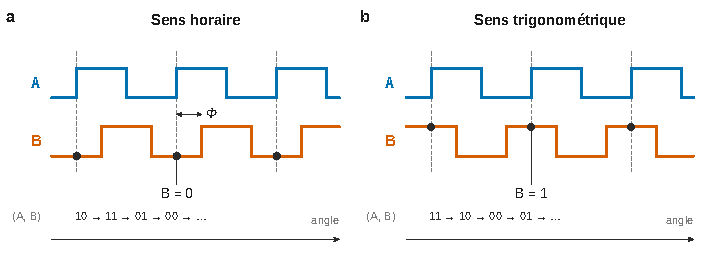
\includegraphics{figures/q1-2-chronogramme-quadrature.pdf}
\caption*{Figure 1 --- chronogrammes des voies A et B dans les deux sens ; B lu au
front montant de A donne le sens}
\end{figure}

On peut aussi suivre les transitions du couple \((A,B)\) : \(00 \to 10 \to 11 \to 01\) dans un sens, et l'ordre inverse dans l'autre. Un compteur-décompteur incrémente ou décrémente selon la transition observée. Avec une seule voie, on compterait les impulsions sans savoir dans quel sens, ce qui est inutilisable pour un asservissement de position.

\begin{methode}

Décoder une quadrature revient à échantillonner une voie sur les fronts de l'autre. Un chronogramme pour chaque sens rend la réponse indiscutable.

\end{methode}

\hypertarget{question-1.3}{%
\subsection{Question 1.3}\label{question-1.3}}

\begin{indication}{1}

Partez de la force subie par des charges en mouvement dans un champ magnétique.

\end{indication}

\begin{indication}{2}

Écrivez l'équilibre en régime permanent entre la force électrique due aux charges accumulées et la force magnétique. Exprimez ensuite la vitesse des porteurs en fonction du courant.

\end{indication}

\begin{indication}{3}

Pour la détection, pensez à ce qui change quand un pôle Nord puis un pôle Sud défilent devant le capteur, et à la mise en forme logique du signal.

\end{indication}

\hypertarget{solution-2}{%
\subsubsection{Solution}\label{solution-2}}

\textbf{Effet Hall.} Une plaquette semi-conductrice d'épaisseur \(e\) et de largeur \(\ell\) est parcourue par un courant \(I\) suivant \(\vec x\). Elle est plongée dans un champ \(\vec B = B\,\vec z\).

Les porteurs de charge \(q\), de densité \(n\), se déplacent à la vitesse \(\vec v = v\,\vec x\). Ils subissent la force de Lorentz, dirigée suivant \(\vec y\) :

\equationajustee{\vec F = q\,\vec v\wedge\vec B}

Ils s'accumulent sur une face latérale, et la face opposée se charge en sens contraire. Le champ transverse \(E_H\) croît jusqu'à l'équilibre avec la force magnétique. Avec l'expression du courant :

\equationajustee{\begin{aligned}
q\,E_H &= q\,v\,B \\
I &= n\,q\,v\,\ell\,e
\end{aligned}}

On en déduit la tension de Hall :

\equationajustee{\begin{aligned}
U_H &= \ell\,E_H \\
&= \frac{I\,B}{n\,q\,e}
\end{aligned}}

\equationajustee{\boxed{U_H = \frac{I\,B}{n\,q\,e}}}

À courant constant, la tension de Hall est \textbf{proportionnelle au champ}. Le capteur mesure le champ sans contact, même à vitesse nulle.

\textbf{Détection d'un aimant.} Le rotor porte des aimants dont les pôles Nord et Sud alternent devant le capteur fixe. À chaque changement de pôle, le champ, et donc \(U_H\), change de signe. Un comparateur à hystérésis (trigger de Schmitt) intégré au capteur transforme cette tension en signal logique : niveau haut devant un pôle, niveau bas devant l'autre. L'hystérésis supprime les rebonds dus au bruit au voisinage du seuil. Deux capteurs décalés d'un quart de pas polaire fournissent \(A\) et \(B\) en quadrature. Un troisième capteur, en regard d'un repère unique, fournit l'index.

\begin{piege}

Ne confondez pas effet Hall et induction. Un capteur inductif ne voit que les variations du champ et ne fournit plus de signal à l'arrêt. Le capteur à effet Hall, lui, mesure le champ lui-même, même à l'arrêt.

\end{piege}

\hypertarget{question-1.4}{%
\subsection{Question 1.4}\label{question-1.4}}

\begin{indication}{1}

Remontez la chaîne cinématique du codeur jusqu'à la tige du vérin, en notant où est monté le codeur.

\end{indication}

\begin{indication}{2}

L'énoncé insiste sur la quadrature : combien de fronts exploitables compte-t-on par période ?

\end{indication}

\begin{indication}{3}

Lisez correctement la référence de la vis : quel nombre est le diamètre, lequel est le pas ?

\end{indication}

\hypertarget{solution-3}{%
\subsubsection{Solution}\label{solution-3}}

\begin{itemize}
\tightlist
\item
  \textbf{Quadrature} : chaque voie délivre \(N = 64\) impulsions par tour. Avec les fronts montants et descendants des deux voies, on dispose de \(4N = 256\) incréments par tour de moteur.
\item
  \textbf{Réducteur} : le codeur est sur l'arbre moteur, en amont du réducteur de rapport 30. Un tour de vis correspond donc à \(30\times 256 = 7680\) incréments.
\item
  \textbf{Vis} : la référence DST-LS-10X12 désigne une vis de diamètre 10 mm et de \textbf{pas \(p = 12\) mm}. Un tour de vis fait avancer la tige de 12 mm.
\end{itemize}

\equationajustee{\begin{aligned}
\Delta x &= \frac{p}{4Nk} \\
&= \frac{12}{4\times 64\times 30}\ \text{mm} \\
&= \frac{12}{7680}\ \text{mm}
\end{aligned}}

\equationajustee{\boxed{\Delta x \approx 1{,}56\ \mu\text{m}}}

Il s'agit d'une résolution, c'est-à-dire du plus petit déplacement mesurable. Ce n'est pas une précision de positionnement : les jeux du réducteur et de l'écrou la dégradent.

\begin{piege}

Chaque oubli coûte un facteur : sans la quadrature, on trouve 6,25 µm ; sans le réducteur, 47 µm. Et confondre le pas (12) avec le diamètre (10) fausse tout le calcul.

\end{piege}

\begin{jury}

Rapport 2026 (p.~2) : « le calcul de la résolution d'un déplacement n'est pas maîtrisé ». Écrire la chaîne complète (fronts par tour, rapport du réducteur, pas de la vis) avant l'application numérique permet d'obtenir les points de la démarche même en cas d'erreur de calcul.

\end{jury}

\hypertarget{question-1.5}{%
\subsection{Question 1.5}\label{question-1.5}}

\begin{indication}{1}

Passez de la vitesse du moteur à celle de la vis, puis à la vitesse de translation de la tige.

\end{indication}

\begin{indication}{2}

Faites attention aux unités : des tours par minute, mais une durée attendue en secondes.

\end{indication}

\hypertarget{solution-4}{%
\subsubsection{Solution}\label{solution-4}}

\equationajustee{\begin{aligned}
N_v &= \frac{N_m}{k} \\
&= \frac{1000}{30} \approx 33{,}3\ \text{tr/min} \\
V &= N_v\,p \\
&= 400\ \text{mm/min} \approx 6{,}67\ \text{mm/s}
\end{aligned}}

On suppose la vitesse constante et on néglige les phases d'accélération et de freinage :

\equationajustee{\begin{aligned}
t_v &= \frac{c}{V} \\
&= \frac{100\times 60}{400}\ \text{s}
\end{aligned}}

\equationajustee{\boxed{t_v = 15\ \text{s}}}

\hypertarget{question-1.6}{%
\subsection{Question 1.6}\label{question-1.6}}

\begin{indication}{1}

Le DR V est un diagramme d'états avec des barres de synchronisation. Comment se combinent les durées de branches qui s'exécutent en parallèle ?

\end{indication}

\begin{indication}{2}

Repérez de combien le robot avance au cours d'un cycle complet.

\end{indication}

\hypertarget{solution-5}{%
\subsubsection{Solution}\label{solution-5}}

On remplace l'activité des vérins par sa durée \(t_v = 15\) s (Q1.5). Les branches parallèles se combinent par leur \textbf{maximum}. Les contrôles d'appui ne sont pas chiffrés : on les suppose plus courts que les branches avec lesquelles ils s'exécutent.

\begin{itemize}
\tightlist
\item
  Séquence initiale : repliement des bras AV (3 s), déploiement des vérins (15 s), déploiement des bras AV (7 s). Total : \textbf{25 s}.
\item
  Fourche 1 : en parallèle avec le contrôle d'appui AV, on enchaîne le repliement des bras AR (3 s), le repliement des vérins (15 s) et le déploiement des bras AR (7 s). Vient ensuite la fourche 2, où le contrôle d'appui AR s'exécute en parallèle avec la prise de vues (10 s). Total : \(3 + 15 + 7 + 10 =\) \textbf{35 s}.
\end{itemize}

Durée d'un cycle : \(T = 25 + 35 = 60\) s. Pendant un cycle, le module avant avance de 100 mm, puis le module arrière le rejoint : le robot progresse de 100 mm.

\equationajustee{\begin{aligned}
D &= \frac{3600}{60}\times 0{,}1\ \text{m} \\
&= 6\ \text{m}
\end{aligned}}

\equationajustee{\boxed{D = 6\ \text{m en 1 h}}}

Ce résultat découle du modèle cinématique du cycle. Il ne s'obtient pas en reprenant la vitesse de 0,1 m/s du DR I : la question demande de vérifier cette performance, pas de la recopier.

On compare ce résultat aux 360 m/h du DR I. Ces 360 m/h correspondent au mode \textbf{hybride} : le robot est porté par le courant (0,1 m/s pour un flux de 0,3 m/s). Les 6 m/h correspondent au mode \textbf{automoteur} seul, par avances successives.

\begin{methode}

Dans un diagramme d'états, la durée totale se calcule sur le \textbf{chemin critique} : on additionne les étapes en série et on prend le maximum des branches parallèles.

\end{methode}

\begin{piege}

Multiplier la vitesse de 0,1 m/s du DR I par une heure donne 360 m : c'est recopier la performance annoncée, pas la vérifier.

\end{piege}

\begin{jury}

Rapport 2026 (p.~2) : Q1.5 et Q1.6 ont donné lieu à « une erreur de fond quasi systématique ». En effet, « les candidats ont utilisé les performances fournies dans le document ressource pour faire leur calcul et non pas vérifier ces performances par un modèle cinématique du déplacement ». Bilan : 65 \% de zéros et 10 \% de bonnes réponses. Une fois le modèle établi, l'écart avec les 360 m/h doit être commenté.

\end{jury}

\hypertarget{question-1.7}{%
\subsection{Question 1.7}\label{question-1.7}}

\begin{indication}{1}

Faites un schéma plan : chaque point d'attache d'un vérin se déplace sur une droite parallèle à \(\vec x\).

\end{indication}

\begin{indication}{2}

Si les deux points d'attache appartenaient à la même pièce rigide, quelle distance resterait constante ? Est-ce compatible avec une rotation de la platine ?

\end{indication}

\hypertarget{solution-6}{%
\subsubsection{Solution}\label{solution-6}}

Les deux vérins sont en glissière de direction \(\vec x\) par rapport à la vertèbre. Leurs points d'attache \(P_1\) et \(P_2\) se déplacent donc sur deux droites parallèles à \(\vec x\), distantes de l'entraxe \(e\).

Supposons-les reliés tous les deux à la platine par des pivots d'axe \(\vec z\). La distance \(L = P_1P_2\) serait alors fixée par la platine, solide indéformable. Au montage, \(P_1P_2\) est perpendiculaire à \(\vec x\), donc \(L = e\).

Si la platine tourne de \(\theta\) autour de \(\vec z\), la projection de \(\overrightarrow{P_1P_2}\) sur \(\vec y\) vaut \(L\cos\theta\). Elle doit rester égale à l'entraxe \(e\) :

\equationajustee{\begin{aligned}
L\cos\theta &= L \\
\Longrightarrow\quad \cos\theta &= 1 \\
\Longrightarrow\quad \theta &= 0
\end{aligned}}

\textbf{La rotation de la platine est impossible.} Le module ne peut plus être orienté, les deux vérins doivent sortir de la même longueur. Si on les commande différemment, le mécanisme se bloque et les liaisons se mettent en contrainte.

\begin{figure}[H]
\centering
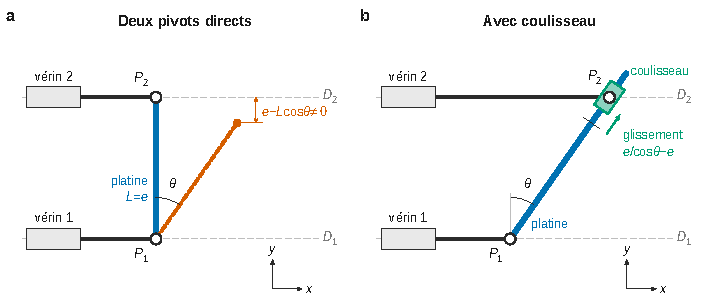
\includegraphics{figures/q1-7-platine-deux-pivots.pdf}
\caption*{Figure 2 --- vue de dessus : deux pivots directs bloquent la rotation de
la platine, le coulisseau la libère}
\end{figure}

La solution est de libérer, côté vérin 2, un déplacement suivant \(\vec y\) par rapport à la platine. C'est le rôle du \textbf{coulisseau}, en glissière de direction \(\vec y\) sur la platine. Le point \(P_2\) reste sur la droite du vérin 2, et \(P_1P_2\) devient \(e/\cos\theta\). Le coulisseau glisse donc le long de la platine de :

\equationajustee{\frac{e}{\cos\theta} - e \approx \frac{e\,\theta^2}{2}}

\begin{piege}

Une étude en vitesses au voisinage de \(\theta = 0\) laisse croire qu'une rotation reste possible, car cette configuration est \textbf{singulière} : au premier ordre, le rang de la fermeture chute. Seul le raisonnement en déplacements finis tranche.

\end{piege}

\begin{jury}

Rapport 2026 (p.~2) : le schéma attendu « a rarement été pertinent et se limitait parfois à une recopie des figures du sujet sans illustrer le problème technique à identifier ». Le jury souligne « la difficulté à proposer un schéma compréhensible par lui-même ». Un bon schéma montre les deux droites des vérins, la platine tournée et la distance qui ne peut pas rester constante.

\end{jury}

\hypertarget{question-1.8}{%
\subsection{Question 1.8}\label{question-1.8}}

\begin{indication}{1}

Commencez par le graphe des liaisons du DR VI. N'oubliez pas la liaison entre la platine et le module.

\end{indication}

\begin{indication}{2}

Associez chaque mobilité à l'actionneur qui la commande et à la fonction qu'elle remplit dans le déplacement du robot.

\end{indication}

\hypertarget{solution-7}{%
\subsubsection{Solution}\label{solution-7}}

Les classes d'équivalence sont : 0 vertèbre, 1 vérin 1, 2 vérin 2, 3 coulisseau, 4 platine, 5 module. Les liaisons sont : 0-1 et 0-2 glissières \(\vec x\), 1-4 pivot \(\vec z\), 2-3 pivot \(\vec z\), 3-4 glissière \(\vec y\), 4-5 pivot \(\vec x\). Le graphe comporte une boucle (0-1-4-3-2-0) et une branche (4-5).

\begin{figure}[H]
\centering
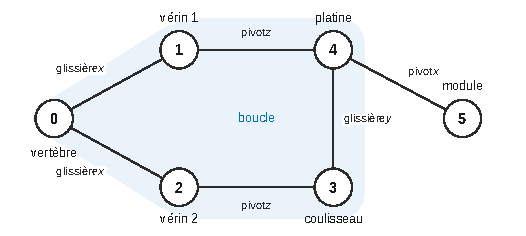
\includegraphics{figures/q1-8-graphe-liaisons.pdf}
\caption*{Figure 3 --- graphe des liaisons de la fixation des vérins : une boucle
0-1-4-3-2-0 et une branche 4-5}
\end{figure}

Les trois mobilités utiles sont :

\begin{itemize}
\tightlist
\item
  \textbf{translation de la platine et du module suivant \(\vec x\)}, par sortie identique des deux vérins, pour avancer ;
\item
  \textbf{rotation de la platine autour de \(\vec z\)}, par sortie différentielle des vérins, pour orienter le module dans le plan de la courbure ;
\item
  \textbf{rotation du module autour de \(\vec x\)}, commandée par le dispositif de rotation axiale, pour changer de plan de courbure.
\end{itemize}

Le glissement du coulisseau n'est pas une mobilité indépendante : il est imposé par les courses des deux vérins.

\hypertarget{question-1.9}{%
\subsection{Question 1.9}\label{question-1.9}}

\begin{indication}{1}

Comptez les liaisons, les pièces et les cycles indépendants, puis appliquez \(m - h = I_c - E_c\).

\end{indication}

\begin{indication}{2}

Pour savoir \emph{quelles} inconnues sont hyperstatiques (ce qui servira pour Q1.10), regardez quelles équations de fermeture sont identiquement nulles.

\end{indication}

\hypertarget{solution-8}{%
\subsubsection{Solution}\label{solution-8}}

Le graphe compte 6 liaisons et 6 classes d'équivalence, et chaque liaison a un degré de liberté :

\equationajustee{\begin{aligned}
\gamma &= L - N + 1 \\
&= 6 - 6 + 1 = 1 \\
E_c &= 6\,\gamma = 6 \\
I_c &= 6
\end{aligned}}

Avec la mobilité \(m = 3\) donnée par l'énoncé :

\equationajustee{\begin{aligned}
h &= m - I_c + E_c \\
&= 3 - 6 + 6
\end{aligned}}

\equationajustee{\boxed{h = 3}}

Vérification par la fermeture cinématique de la boucle. Les rotations sont toutes d'axe \(\vec z\), et les translations sont toutes dans le plan \((\vec x,\vec y)\).

Seules trois équations sont utiles : la rotation suivant \(\vec z\) et les translations suivant \(\vec x\) et \(\vec y\). Le rang vaut \(r_c = 3\), d'où \(h = 6 - 3 = 3\).

La mobilité de la boucle vaut \(5 - 3 = 2\). La branche ajoute 1, d'où \(m = 3\).

Les équations inutilisées désignent les inconnues hyperstatiques : \textbf{rotations autour de \(\vec x\) et de \(\vec y\), translation suivant \(\vec z\)}. Le mécanisme est plan mais réalisé avec des liaisons spatiales. Il faut donc des pivots rigoureusement parallèles entre eux et perpendiculaires au plan de glissement.

\begin{methode}

Pour un mécanisme plan modélisé dans l'espace, chaque boucle apporte en général 3 inconnues hyperstatiques : les deux rotations hors du plan et la translation normale au plan.

\end{methode}

\hypertarget{question-1.10}{%
\subsection{Question 1.10}\label{question-1.10}}

\begin{indication}{1}

Relisez le DR VI : entre quelles pièces se trouve réellement la glissière ? Signalez l'imprécision de l'énoncé et poursuivez.

\end{indication}

\begin{indication}{2}

Ajoutez exactement les degrés de liberté qui correspondent aux équations inutilisées de Q1.9.

\end{indication}

\begin{indication}{3}

Identifiez dans le tableau des liaisons usuelles celle qui possède ces quatre degrés de liberté, et donnez ses éléments géométriques.

\end{indication}

\hypertarget{solution-9}{%
\subsubsection{Solution}\label{solution-9}}

Sur le DR VI, le vérin 2 est en \textbf{pivot} avec le coulisseau, et la \textbf{glissière} de direction \(\vec y\) relie le coulisseau à la platine. C'est cette liaison (un seul degré de liberté, \(T_y\)) que l'on modifie, en signalant l'imprécision du libellé. Le raisonnement reste le même quelle que soit la liaison retenue : on libère exactement les mobilités associées aux inconnues hyperstatiques de Q1.9.

Il faut lui ajouter :

\equationajustee{\boxed{T_z,\quad R_x,\quad R_y}}

La liaison obtenue a pour degrés de liberté \(\{T_y, T_z, R_x, R_y\}\). \textbf{C'est une liaison linéaire rectiligne de normale \(\vec x\), dont la ligne de contact est dirigée par \(\vec y\).} Elle laisse libres les deux translations dans le plan tangent \((\vec y,\vec z)\), la rotation autour de la normale et la rotation autour de la ligne de contact. Elle transmet une résultante suivant \(\vec x\) et un moment suivant \(\vec z\).

Vérification : \(I_c = 4 + 4 + 1 = 9\), le rang de la fermeture vaut 6, donc \(h = 0\) et \(m = 9 - 6 = 3\).

\begin{piege}

Un pivot glissant n'ajoute que \(R_y\) (ou \(R_x\)), et il reste alors \(h = 2\). Un appui plan ne libère pas \(R_y\), et il reste \(h = 1\). Il faut partir des inconnues hyperstatiques identifiées, et non essayer les liaisons au hasard.

\end{piege}

\begin{jury}

Rapport 2026 (p.~2) : « Le sujet comportait une confusion sur la liaison à étudier pour rendre le mécanisme isostatique ». Les correcteurs en ont tenu compte « en évaluant uniquement le raisonnement peu importe à quelle liaison il était appliqué ». Signaler l'ambiguïté, choisir une liaison et dérouler le raisonnement complet est donc la bonne conduite, conforme à la consigne de la première page du sujet.

\end{jury}

\hypertarget{question-1.11}{%
\subsection{Question 1.11}\label{question-1.11}}

\begin{indication}{1}

Deux rails et deux patins vissés : si chacun portait sur de larges plans et contre des épaulements, combien de fois la même position serait-elle imposée ?

\end{indication}

\begin{indication}{2}

Hiérarchisez : un appui plan de référence, une butée latérale pour un seul rail (et un seul patin), et des dégagements partout ailleurs.

\end{indication}

\hypertarget{solution-10}{%
\subsubsection{Solution}\label{solution-10}}

Le guidage du coulisseau est réalisé par deux rails vissés sur la platine et deux patins vissés sur le coulisseau. Pour limiter l'hyperstatisme, on restreint et on hiérarchise les surfaces de mise en position. Les surfaces surlignées en rouge sont les suivantes.

\textbf{Coupe A-A} (perpendiculaire aux rails) :

\begin{itemize}
\tightlist
\item
  \textbf{platine} : sous chaque rail, une \textbf{portée plane étroite} de normale \(\vec x\), de la largeur de la semelle du rail. Ces portées sont coplanaires et usinées dans la même opération, et la matière comprise entre elles est dégagée. Un \textbf{épaulement latéral} de normale \(\vec z\) existe \textbf{sous un seul rail} (rail de référence). Le second rail n'a pas de butée latérale : ses vis passent dans des trous avec jeu, et il s'aligne au montage ;
\item
  \textbf{coulisseau} : deux portées planes étroites coplanaires de normale \(\vec x\), une par patin. Un seul épaulement latéral de normale \(\vec z\), pour le patin de référence.
\end{itemize}

\textbf{Coupe B-B} (le long du rail de référence) : sous le rail, la platine ne porte qu'au droit des deux vis CHC, sur deux plages coplanaires de longueur limitée, et la matière est dégagée entre elles. Le coulisseau porte sur le patin par une plage limitée à l'emprise du patin.

On surligne en rouge les portées planes et les deux épaulements de référence. On ne surligne pas les portées des têtes de vis (surfaces de serrage) ni les dégagements. Les bossages doivent être réalisables en fraisage, avec un raccordement ou un dégagement d'outil.

\begin{piege}

Surligner les surfaces de serrage sous les têtes de vis est une erreur fréquente. Elles maintiennent la pièce en position, elles ne la mettent pas en position.

\end{piege}

\begin{jury}

Rapport 2026 (p.~2) : le dessin de cette question était « souvent inachevé et limité au prolongement de quelques traits ». Il faut dessiner les deux pièces complètes dans les deux coupes, avec les dégagements, avant de surligner.

\end{jury}

\hypertarget{question-1.12}{%
\subsection{Question 1.12}\label{question-1.12}}

\begin{indication}{1}

Lisez les deux points extrêmes de la loi E/S du DR VIII et la définition de \(\rho\) : où le patin s'ajoute-t-il ?

\end{indication}

\begin{indication}{2}

La loi est décroissante. Laquelle des deux bornes correspond aux bras repliés ?

\end{indication}

\hypertarget{solution-11}{%
\subsubsection{Solution}\label{solution-11}}

\(\rho\) est la distance entre le centre et le support du patin. Le patin d'épaisseur \(\delta\) s'ajoute radialement, donc \(D = 2(\rho+\delta)\).

Les deux bornes de la loi E/S sont :

\begin{itemize}
\tightlist
\item
  bras repliés : \(\alpha = 42^\circ\) et \(\rho = 54{,}16\) mm ;
\item
  bras déployés : \(\alpha = 7{,}5^\circ\) et \(\rho = 114{,}81\) mm.
\end{itemize}

\equationajustee{\begin{aligned}
D_{\min} &= 2\,(54{,}16+27) \\
D_{\max} &= 2\,(114{,}81+27)
\end{aligned}}

\equationajustee{\boxed{\begin{aligned}
D_{\min} &\approx 162\ \text{mm} \\
D_{\max} &\approx 284\ \text{mm}
\end{aligned}}}

\begin{itemize}
\tightlist
\item
  150 mm : \textbf{non}, car \(D_{\min} > 150\) mm.
\item
  200 mm : \textbf{oui}, avec \(\rho = 73\) mm, soit \(\alpha \approx 34{,}5^\circ\).
\item
  250 mm : \textbf{oui}, avec \(\rho = 98\) mm, soit \(\alpha \approx 21^\circ\).
\end{itemize}

On remarque que \(D_{\max} < 300\) mm, alors que le DR I annonce aussi des conduites de 300 mm : celles-ci demandent une autre version de cassette.

\begin{piege}

Oublier l'épaisseur des patins inverse la conclusion : on trouverait alors 108 et 230 mm, ce qui laisserait croire que le robot passe dans 150 mm mais pas dans 250 mm. Le rapport 2026 relève aussi des confusions entre diamètre et rayon : \(\rho\) est un rayon, et on le compare à la moitié du diamètre de la conduite.

\end{piege}

\hypertarget{question-1.13}{%
\subsection{Question 1.13}\label{question-1.13}}

\begin{indication}{1}

Les arbres intermédiaires sont-ils en pivot avec le bâti ou avec un porte-satellites mobile ? Cela décide de la méthode de calcul.

\end{indication}

\begin{indication}{2}

Un engrènement extérieur inverse le sens de rotation, un engrènement intérieur le conserve. Suivez les deux chemins de puissance, de \(Z_1\) jusqu'à chacune des couronnes.

\end{indication}

\begin{indication}{3}

Pour conclure sur le déploiement, comparez les signes et les modules des deux rapports.

\end{indication}

\hypertarget{solution-12}{%
\subsubsection{Solution}\label{solution-12}}

Tous les arbres intermédiaires sont en pivot avec le bâti : le train fonctionne \textbf{à axes fixes}. \(Z_3\) et \(Z_7\) sont les dentures intérieures des couronnes.

\equationajustee{\frac{\omega_{c1}}{\omega_e} = \left(-\frac{Z_1}{Z_2}\right)\left(+\frac{Z_2}{Z_3}\right) = -\frac{15}{75}}

\equationajustee{\frac{\omega_{c2}}{\omega_e} = \left(-\frac{Z_1}{Z_2}\right)\left(-\frac{Z_4}{Z_5}\right)\left(+\frac{Z_6}{Z_7}\right) = \left(-\frac12\right)(-1)\left(\frac25\right)}

\equationajustee{\boxed{\begin{aligned}
\frac{\omega_{c1}}{\omega_e} &= -\frac15 \\
\frac{\omega_{c2}}{\omega_e} &= +\frac15
\end{aligned}}}

Ces rapports sont pris par rapport à l'arbre d'entrée du train. Par rapport à l'arbre moteur, ils valent \(\mp 1/980\).

Les deux couronnes tournent \textbf{à la même vitesse et en sens opposés}. \textbf{Le déploiement est donc assuré}, et il est symétrique. La roue 5 est une roue intermédiaire : elle inverse le sens sans changer le module du rapport. Contrôle de géométrie : \(Z_3 = Z_1 + 2Z_2\), et les deux arbres intermédiaires sont à la même distance de l'axe, \(m(Z_1+Z_2)/2 = m(Z_7-Z_6)/2\), où \(m\) est le module.

\begin{piege}

La formule de Willis ne s'applique pas ici, puisqu'il n'y a pas de porte-satellites mobile. Et compter un engrènement intérieur comme extérieur donnerait deux couronnes tournant dans le même sens, donc pas de déploiement.

\end{piege}

\begin{jury}

Rapport 2026 (p.~2) : « l'établissement des rapports des vitesses a posé de grosses difficultés. Le fait que les deux couronnes tournent à des vitesses opposées n'a pas été une évidence, empêchant une prise de recul sur les propositions de réponses. » Le signe de chaque rapport est donc la justification attendue pour conclure sur le déploiement.

\end{jury}

\hypertarget{question-1.14}{%
\subsection{Question 1.14}\label{question-1.14}}

\begin{indication}{1}

Déterminez d'abord, sur la courbe du DR VIII, l'angle \(\alpha\) pour lequel les patins touchent une paroi de 250 mm.

\end{indication}

\begin{indication}{2}

Regardez sur la figure du DR VIII entre quels points l'angle \(\alpha\) est mesuré : à quelle couronne chacun de ces points est-il lié ?

\end{indication}

\begin{indication}{3}

Contrôlez votre hypothèse avec les « 7 s pour une canalisation de 300 mm » du DR V. À 300 mm, où en est le déploiement ?

\end{indication}

\hypertarget{solution-13}{%
\subsubsection{Solution}\label{solution-13}}

\textbf{Angle final.} Pour une conduite de 250 mm, \(\rho_f = 125 - 27 = 98\) mm. La courbe passe par \(\rho = 100\) mm en \(\alpha = 20^\circ\), et on lit \(\alpha_f \approx 21^\circ\). Bras repliés : \(\alpha_i = 42^\circ\). D'où \(\Delta\alpha \approx 21^\circ\).

\textbf{Rotation des couronnes.} \(\alpha\) est l'angle, vu du centre, entre les deux articulations du pantographe, chacune portée par une couronne. Les couronnes tournant de \(\pm\Delta\theta\), on a \(\Delta\alpha = 2\Delta\theta\).

\textbf{Durée.} La vitesse de chaque couronne vaut \(N_e/5 = 0{,}4\) tr/min, soit \(144\ ^\circ\)/min ou \(2{,}4\ ^\circ\)/s.

\equationajustee{\begin{aligned}
t_d &= \frac{\Delta\alpha}{2\times 2{,}4} \\
&= \frac{21}{4{,}8}\ \text{s}
\end{aligned}}

\equationajustee{\boxed{t_d\approx 4{,}4\ \text{s}}}

Avec une incertitude de lecture de \(\pm 0{,}5^\circ\), on obtient un temps compris entre 4,3 et 4,5 s.

\textbf{Contrôle.} Le déploiement complet (\(42^\circ\to 7{,}5^\circ\)) dure \(34{,}5/4{,}8 \approx 7{,}2\) s. Or dans une conduite de 300 mm, les bras vont en butée sans toucher la paroi (\(\rho_{\max} + \delta < 150\) mm). On retrouve donc les 7 s du DR V, ce qui valide la relation \(\Delta\alpha = 2\Delta\theta\). Avec \(\Delta\theta = \Delta\alpha\), on aurait obtenu 14,4 s.

\begin{methode}

Quand une hypothèse cinématique est incertaine, cherchez une donnée du dossier qui permet de la tester. Ici, la durée de 7 s fournit ce test.

\end{methode}

\hypertarget{partie-2-industrialisation-de-la-couronne}{%
\section{Partie 2 --- Industrialisation de la couronne}\label{partie-2-industrialisation-de-la-couronne}}

On part du dessin de définition de la couronne (spécifications GPS), on choisit un matériau par la méthode d'Ashby, puis on compare deux processus de fabrication : l'usinage seul, et la fabrication additive suivie d'usinage. La partie se termine par l'orientation des pièces sur le plateau de fabrication additive et par une gamme d'usinage sur tour 3 axes. Il faut savoir lire un dessin, écrire un indice de performance et connaître les procédés.

\textbf{Lecture préalable du DR X, indispensable :}

\begin{itemize}
\tightlist
\item
  \textbf{A} est la face plane d'extrémité de la couronne.
\item
  \textbf{B} est l'axe du cylindre extérieur Ø62,4 ± 0,01, voisin de A et perpendiculaire à A à Ø0,01 près.
\item
  \textbf{C} est l'axe du cylindre extérieur Ø63,5, la portée du roulement, qui porte aussi la cylindricité 0,005 et Ra 0,8.
\item
  Le battement 0,02 / C est indiqué par une flèche parallèle à l'axe, qui pointe la face plane de l'épaulement servant d'appui au roulement.
\end{itemize}

\hypertarget{question-2.1}{%
\subsection{Question 2.1}\label{question-2.1}}

\begin{indication}{1}

Pour chaque cadre, commencez par le type (forme, orientation, position, battement), puis repérez sur le DR X \textbf{quelle surface} porte la flèche.

\end{indication}

\begin{indication}{2}

Pour le battement, regardez la direction de la flèche : elle donne la direction de mesure. Une flèche parallèle à l'axe qui touche une face plane indique-t-elle un battement radial ou axial ?

\end{indication}

\begin{indication}{3}

Dans la fiche, distinguez bien la référence simple d'un système de références ordonné, et la zone simple d'une zone composée.

\end{indication}

\hypertarget{solution-14}{%
\subsubsection{Solution}\label{solution-14}}

\textbf{(a) Cylindricité 0,005}

\begin{longtable}[]{@{}
  >{\raggedright\arraybackslash}p{(\columnwidth - 2\tabcolsep) * \real{0.3978}}
  >{\raggedright\arraybackslash}p{(\columnwidth - 2\tabcolsep) * \real{0.5722}}@{}}
\toprule\noalign{}
\begin{minipage}[b]{\linewidth}\raggedright
Rubrique de la fiche
\end{minipage} & \begin{minipage}[b]{\linewidth}\raggedright
Contenu
\end{minipage} \\
\midrule\noalign{}
\endhead
\bottomrule\noalign{}
\endlastfoot
Type & \textbf{Forme} \\
Élément tolérancé & \textbf{unique} : la surface cylindrique réelle Ø63,5 (portée du roulement) \\
Élément(s) de référence, référence spécifiée & aucun \\
Zone de tolérance & \textbf{simple} : espace compris entre deux cylindres coaxiaux dont les rayons diffèrent de 0,005 mm \\
Contraintes & aucune : la position, l'orientation et le diamètre de la zone sont libres \\
Conformité & la surface extraite est entièrement contenue dans la zone \\
\end{longtable}

La cylindricité limite en même temps l'ovalisation, le défaut de rectitude des génératrices et la conicité.

\textbf{(b) Battement simple 0,02 par rapport à C} : c'est un battement \textbf{axial}.

\begin{longtable}[]{@{}
  >{\raggedright\arraybackslash}p{(\columnwidth - 2\tabcolsep) * \real{0.2395}}
  >{\raggedright\arraybackslash}p{(\columnwidth - 2\tabcolsep) * \real{0.7305}}@{}}
\toprule\noalign{}
\begin{minipage}[b]{\linewidth}\raggedright
Rubrique de la fiche
\end{minipage} & \begin{minipage}[b]{\linewidth}\raggedright
Contenu
\end{minipage} \\
\midrule\noalign{}
\endhead
\bottomrule\noalign{}
\endlastfoot
Type & \textbf{Battement} (simple, axial) \\
Élément tolérancé & \textbf{unique} : la \textbf{face plane d'épaulement} qui sert d'appui au roulement, analysée ligne par ligne (chaque ligne circulaire est l'intersection de la face avec un cylindre de mesure coaxial à C) \\
Élément de référence & \textbf{unique} : la surface cylindrique Ø63,5 \\
Référence spécifiée & \textbf{simple} : l'axe C du cylindre associé (cylindre minimal circonscrit, la surface étant extérieure) \\
Zone de tolérance & \textbf{simple}, appliquée indépendamment à chaque cylindre de mesure : portion de ce cylindre comprise entre deux cercles distants de 0,02 mm \textbf{suivant l'axe} \\
Contraintes & les cylindres de mesure sont coaxiaux à C et les cercles limites perpendiculaires à C (orientation et position par rapport à C). La position axiale de la zone est libre. \\
Conformité & la pièce tournant autour de C, un comparateur palpant la face (déplacement parallèle à l'axe) ne varie pas de plus de 0,02 mm, pour chaque rayon de palpage \\
\end{longtable}

\begin{figure}[H]
\centering
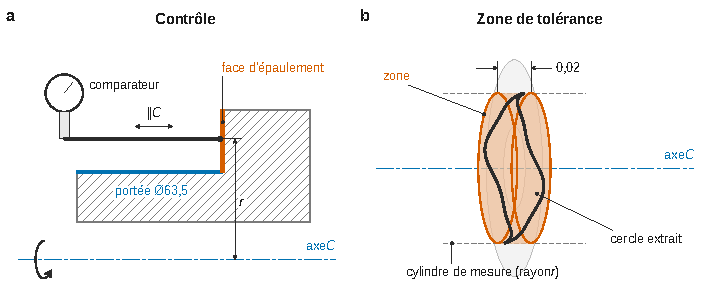
\includegraphics{figures/q2-1-battement-axial.pdf}
\caption*{Figure 4 --- battement axial 0,02 / C : contrôle au comparateur et zone
de tolérance sur un cylindre de mesure}
\end{figure}

Cette spécification garantit que l'appui axial du roulement est perpendiculaire à l'axe de la portée.

\textbf{(c) Localisation Ø0,02 A B}

\begin{longtable}[]{@{}
  >{\raggedright\arraybackslash}p{(\columnwidth - 2\tabcolsep) * \real{0.2604}}
  >{\raggedright\arraybackslash}p{(\columnwidth - 2\tabcolsep) * \real{0.7096}}@{}}
\toprule\noalign{}
\begin{minipage}[b]{\linewidth}\raggedright
Rubrique de la fiche
\end{minipage} & \begin{minipage}[b]{\linewidth}\raggedright
Contenu
\end{minipage} \\
\midrule\noalign{}
\endhead
\bottomrule\noalign{}
\endlastfoot
Type & \textbf{Position} \\
Élément tolérancé & \textbf{unique} : la ligne médiane extraite (axe réel) du cylindre Ø63,5 \\
Éléments de référence & \textbf{multiples} : la face A et la surface cylindrique Ø62,4 \\
Référence spécifiée & \textbf{système} ordonné : A primaire (plan associé du côté libre de la matière), puis B secondaire (axe du cylindre associé au Ø62,4, contraint perpendiculaire à A) \\
Zone de tolérance & \textbf{simple} : cylindre de diamètre 0,02 mm \\
Contraintes & axe de la zone perpendiculaire à A et confondu avec B (distance théorique nulle) \\
Conformité & l'axe extrait est entièrement contenu dans le cylindre Ø0,02 \\
\end{longtable}

\begin{piege}

Le battement ne s'interprète pas toujours comme radial. La direction de la flèche et la nature de la surface pointée (cylindre ou face plane) décident entre battement radial et battement axial. Ici, la flèche est parallèle à l'axe et pointe une face : le battement est axial.

\end{piege}

\begin{methode}

Une spécification de forme n'a jamais de référence. Une spécification d'orientation, de position ou de battement en a toujours une. Le symbole Ø devant la valeur rend la zone cylindrique.

\end{methode}

\begin{jury}

Rapport 2026 (p.~2) : la cylindricité et la localisation ont été mieux traitées, mais « Le battement a été bien moins réussi. » Le jury rappelle que, pour cette épreuve, la feuille GPS utilisée est la version 1 : il faut remplir les rubriques de la fiche du cahier réponse, en rayant les mentions inutiles. Bilan : 21 \% de bonnes réponses.

\end{jury}

\hypertarget{question-2.2}{%
\subsection{Question 2.2}\label{question-2.2}}

\begin{indication}{1}

Calculez les deux dimensions limites, puis rappelez ce que mesure l'opérateur de taille par défaut de l'ISO 14405-1.

\end{indication}

\begin{indication}{2}

Une pièce réelle a-t-elle « un » diamètre ? Que dit le principe d'indépendance sur la forme ?

\end{indication}

\hypertarget{solution-15}{%
\subsubsection{Solution}\label{solution-15}}

\equationajustee{\begin{aligned}
d_{\max} &= 63{,}512\ \text{mm} \\
d_{\min} &= 63{,}493\ \text{mm} \\
IT &= 19\ \mu\text{m}
\end{aligned}}

L'opérateur par défaut est la \textbf{taille locale entre deux points} : on mesure la distance entre deux points opposés de la surface extraite, dans toutes les sections et toutes les directions.

\equationajustee{\boxed{\forall\ \text{paire de points \text{opposés}} :\ 63{,}493\le d_{2\text{pts}}\le 63{,}512\ \text{mm}}}

D'après le \textbf{principe d'indépendance} (ISO 8015), cette cote n'impose aucune forme. Une section trilobée ou un cylindre cintré peuvent être conformes. C'est la cylindricité 0,005 qui limite la forme. Pour lier taille et forme, il aurait fallu l'exigence de l'enveloppe (E cerclé).

\begin{piege}

Écrire « le diamètre doit être compris entre 63,493 et 63,512 mm » ne répond pas à la question, qui porte précisément sur la façon dont la taille est évaluée.

\end{piege}

\begin{jury}

Rapport 2026 (p.~2) : « La notion de bipoints ou de taille n'est pas connue des candidat.es, ce qui a conduit à des réponses erronées dans 75\% des cas. » Le mot attendu est la taille locale entre deux points (bipoint).

\end{jury}

\hypertarget{question-2.3}{%
\subsection{Question 2.3}\label{question-2.3}}

\begin{indication}{1}

Décodez d'abord le symbole graphique : que signifie le triangle fermé par un trait horizontal ?

\end{indication}

\begin{indication}{2}

\(Ra\) est une moyenne sur une longueur de base. Pourquoi faut-il une valeur absolue dans l'intégrale ?

\end{indication}

\hypertarget{solution-16}{%
\subsubsection{Solution}\label{solution-16}}

\begin{itemize}
\tightlist
\item
  Le triangle \textbf{fermé} signifie que l'\textbf{enlèvement de matière est obligatoire} : la surface est usinée, et ne peut pas rester brute de fabrication additive.
\item
  « Ra 0,8 » : l'écart moyen arithmétique du profil de rugosité ne dépasse pas 0,8 µm.
\end{itemize}

\(z(x)\) est l'ordonnée du profil de rugosité (filtré) par rapport à sa ligne moyenne, et \(l_r\) la longueur de base :

\equationajustee{\boxed{Ra = \frac{1}{l_r}\int_0^{l_r}\lvert z(x)\rvert\,\mathrm{d}x}}

Conditions par défaut : coupure \(\lambda_c = 0{,}8\) mm (pour \(0{,}1 < Ra\le 2\) µm), évaluation sur 5 longueurs de base, soit 4 mm, et règle des 16 \%. Un Ra de 0,8 µm correspond à un tournage de finition soigné ou à une rectification.

\begin{piege}

Sans la valeur absolue, l'intégrale est nulle, puisque la ligne moyenne est définie comme celle qui annule la moyenne des écarts.

\end{piege}

\hypertarget{question-2.4}{%
\subsection{Question 2.4}\label{question-2.4}}

\begin{indication}{1}

Passez en revue le milieu de fonctionnement (eau potable sous pression), les sollicitations mécaniques, les contraintes du robot (flottabilité, autonomie) et la production (petite série).

\end{indication}

\begin{indication}{2}

Séparez les critères qui éliminent des matériaux de ceux qui permettent de classer ceux qui restent.

\end{indication}

\hypertarget{solution-17}{%
\subsubsection{Solution}\label{solution-17}}

\begin{enumerate}
\def\labelenumi{\arabic{enumi}.}
\tightlist
\item
  \textbf{Conformité au contact avec l'eau potable}, rappelée par l'énoncé : critère éliminatoire, aucune substance ne doit être relarguée.
\item
  \textbf{Tenue à la corrosion} en eau chlorée sous 20 bars, pour préserver les dentures, les portées et la qualité de l'eau.
\item
  \textbf{Résistance mécanique} \(\sigma_{\max}\) : oreilles en flexion, dentures en flexion et en pression de contact.
\item
  \textbf{Faible masse volumique} \(\rho\) : flottabilité neutre et énergie embarquée.
\item
  \textbf{Mise en œuvre} : usinabilité (IT 19 µm, Ra 0,8) et compatibilité avec la fabrication additive.
\item
  \textbf{Coût}, rapporté à quelques pièces par an.
\end{enumerate}

Les critères 1 et 2 \textbf{trient}, les critères 3 et 4 \textbf{classent} au moyen de l'indice de performance des questions suivantes.

\begin{jury}

Le rapport 2026 (p.~4) conseille de « justifier brièvement, mais systématiquement les démarches et les solutions proposées ». Ici, chaque critère doit être relié au contexte (eau potable, 20 bars, flottabilité, petite série) : un critère cité sans raison rapporte peu.

\end{jury}

\hypertarget{question-2.5}{%
\subsection{Question 2.5}\label{question-2.5}}

\begin{indication}{1}

Volume d'un cylindre, et moment quadratique d'un disque par rapport à un diamètre.

\end{indication}

\hypertarget{solution-18}{%
\subsubsection{Solution}\label{solution-18}}

\equationajustee{\boxed{m = \rho\,\pi\,r^2\,L}}

\equationajustee{\begin{aligned}
I_{Gz} &= \iint_S y^2\,\mathrm{d}S \\
&= \frac{\pi r^4}{4}
\end{aligned}}

\equationajustee{\boxed{I_{Gz} = \frac{\pi r^4}{4}}}

Calcul de \(I_{Gz}\) en coordonnées polaires : \(\displaystyle\int_0^r\!\!\int_0^{2\pi} s^2\sin^2\varphi\; s\,\mathrm{d}\varphi\,\mathrm{d}s = \frac{r^4}{4}\,\pi\).

\begin{piege}

Le moment polaire \(\pi r^4/2\) sert en torsion, pas en flexion.

\end{piege}

\hypertarget{question-2.6}{%
\subsection{Question 2.6}\label{question-2.6}}

\begin{indication}{1}

Le rayon \(r\) n'est pas imposé : c'est lui qui s'adapte au matériau. Éliminez-le entre la condition de résistance et la masse.

\end{indication}

\begin{indication}{2}

Regroupez ensuite les puissances de \(\rho\) et de \(\sigma_{\max}\) d'un côté, celles de \(L\) et de \(F\) de l'autre.

\end{indication}

\hypertarget{solution-19}{%
\subsubsection{Solution}\label{solution-19}}

\equationajustee{\begin{aligned}
F &= \frac{\sigma_{\max}}{Lr}\cdot\frac{\pi r^4}{4} \\
&= \frac{\pi\sigma_{\max}r^3}{4L} \\
\Longrightarrow\quad r &= \left(\frac{4FL}{\pi\sigma_{\max}}\right)^{1/3}
\end{aligned}}

\equationajustee{\begin{aligned}
m &= \rho\pi L r^2 \\
&= \rho\pi L\left(\frac{4FL}{\pi\sigma_{\max}}\right)^{2/3}
\end{aligned}}

\equationajustee{\boxed{m = \underbrace{\frac{\rho}{\sigma_{\max}^{2/3}}}_{f_1}\cdot\underbrace{\pi^{1/3}4^{2/3}L^{5/3}}_{f_2}\cdot\underbrace{F^{2/3}}_{f_3}}\qquad(\pi^{1/3}4^{2/3}\approx 3{,}69)}

À \(L\) et \(F\) imposés, minimiser \(m\) revient à maximiser \(I_p = 1/f_1 = \sigma_{\max}^{2/3}/\rho\), soit \(n = 2/3\).

\begin{methode}

Pour établir un indice de performance : écrire l'objectif (la masse), écrire la contrainte (la résistance), éliminer la variable libre (ici \(r\)), puis séparer les termes qui dépendent du matériau, de la géométrie et du chargement.

\end{methode}

\hypertarget{question-2.7}{%
\subsection{Question 2.7}\label{question-2.7}}

\begin{indication}{1}

Que devient la relation \(\sigma_{\max}^{2/3}/\rho = C\) dans un diagramme log-log ? Quelle est la pente de la droite ?

\end{indication}

\begin{indication}{2}

Dans quel sens faut-il déplacer cette droite pour augmenter \(C\) ? Puis appliquez les critères éliminatoires de Q2.4 aux matériaux qui restent au-dessus.

\end{indication}

\begin{indication}{3}

Pensez aux deux procédés additifs étudiés ensuite : l'un est métallique, l'autre polymère.

\end{indication}

\hypertarget{solution-20}{%
\subsubsection{Solution}\label{solution-20}}

\textbf{Méthode.}

\begin{enumerate}
\def\labelenumi{\arabic{enumi}.}
\tightlist
\item
  À indice constant, on a \(\log\sigma_{\max} = \frac32\log\rho + \text{cte}\). Les matériaux de même performance sont donc alignés sur une \textbf{droite de pente 3/2}, parallèle à la ligne guide \(\sigma_f^{2/3}/\rho\) du DR XI.
\item
  En translatant la droite \textbf{vers le haut et vers la gauche}, on ne garde que les meilleurs matériaux.
\item
  On élimine ensuite ceux qui ne respectent pas les exigences : contact avec l'eau potable, corrosion, fragilité, compatibilité avec les procédés.
\end{enumerate}

\begin{longtable}[]{@{}
  >{\raggedright\arraybackslash}p{(\columnwidth - 8\tabcolsep) * \real{0.1996}}
  >{\raggedright\arraybackslash}p{(\columnwidth - 8\tabcolsep) * \real{0.1629}}
  >{\raggedright\arraybackslash}p{(\columnwidth - 8\tabcolsep) * \real{0.1509}}
  >{\raggedright\arraybackslash}p{(\columnwidth - 8\tabcolsep) * \real{0.0871}}
  >{\raggedright\arraybackslash}p{(\columnwidth - 8\tabcolsep) * \real{0.3695}}@{}}
\toprule\noalign{}
\begin{minipage}[b]{\linewidth}\raggedright
Matériau
\end{minipage} & \begin{minipage}[b]{\linewidth}\raggedright
\(\sigma_f\) (MPa)
\end{minipage} & \begin{minipage}[b]{\linewidth}\raggedright
\(\rho\) (Mg/m³)
\end{minipage} & \begin{minipage}[b]{\linewidth}\raggedright
\(I_p\)
\end{minipage} & \begin{minipage}[b]{\linewidth}\raggedright
Décision
\end{minipage} \\
\midrule\noalign{}
\endhead
\bottomrule\noalign{}
\endlastfoot
CFRP & ≈ 700 & 1,6 & ≈ 49 & écarté : anisotrope, inadapté à une denture, hors des procédés envisagés \\
Céramiques techniques & ≈ 1000 & ≈ 3,2 & ≈ 31 & écartées : fragiles \\
\textbf{Alliages de titane} & ≈ 900 & 4,5 & ≈ 21 & \textbf{retenus} \\
Alliages de magnésium & ≈ 200 & 1,8 & ≈ 19 & écartés : corrosion \\
Alliages d'aluminium & ≈ 300 & 2,7 & ≈ 17 & moins bons que le titane, tenue à la corrosion moyenne \\
\textbf{PEEK} & ≈ 100 & 1,3 & ≈ 17 & \textbf{retenu} \\
Aciers inoxydables & ≈ 500 & 7,8 & ≈ 8 & indice faible \\
\end{longtable}

\textbf{Choix : un alliage de titane (Ti-6Al-4V) pour les métaux, et le PEEK pour les polymères.}

\begin{itemize}
\tightlist
\item
  Le titane : meilleur indice parmi les matériaux admissibles, excellente tenue à la corrosion, compatibilité sanitaire, mise en œuvre par fusion laser sur lit de poudre.
\item
  Le PEEK : indice proche de celui de l'aluminium pour une masse volumique environ deux fois plus faible, qualité contact alimentaire, mise en œuvre par dépôt de fil fondu.
\end{itemize}

\begin{piege}

Retenir deux métaux (par exemple titane et aluminium) ne respecte pas la consigne. Retenir le CFRP parce qu'il est le mieux placé, sans le confronter aux exigences, non plus.

\end{piege}

\begin{jury}

Rapport 2026 (p.~2) : « la majorité des candidat.es ne sait pas exploiter ces graphes de sélection à partir d'un indice de performance, ce qui conduit à des propositions de matériaux farfelues (bétons, mousse, etc.) ». La droite de pente 3/2 tracée sur le diagramme, puis le tri par les exigences fonctionnelles, constituent la méthodologie demandée. Bilan de Q2.4 à Q2.8 : 24 \% de bonnes réponses.

\end{jury}

\hypertarget{question-2.8}{%
\subsection{Question 2.8}\label{question-2.8}}

\begin{indication}{1}

Écrivez le coût unitaire en séparant ce qui est payé une fois (l'outillage) de ce qui est payé à chaque pièce.

\end{indication}

\begin{indication}{2}

Passez en revue les grandes familles de procédés et repérez celles qui exigent un moule ou une matrice dédiée.

\end{indication}

\hypertarget{solution-21}{%
\subsubsection{Solution}\label{solution-21}}

\(C_u = C_{\text{outillage}}/n + c_{\text{\text{matière}}} + c_{\text{\text{opératoire}}}\). Pour \(n\) de l'ordre de quelques unités, le terme d'outillage domine. \textbf{Tous les procédés à outillage dédié sont exclus} :

\begin{itemize}
\tightlist
\item
  l'injection plastique (moule complexe à cause de la denture intérieure, et PEEK mis en œuvre vers 380 °C) ;
\item
  la fonderie en moule métallique et le moulage de précision (et le titane, très réactif à chaud, est difficile à couler) ;
\item
  le forgeage et le matriçage (matrices dédiées, et pas de denture directe) ;
\item
  le frittage et le moulage par injection de poudres (outillage et mise au point de cycle) ;
\item
  le découpage, l'emboutissage et l'extrusion (outillages dédiés, géométrie inaccessible).
\end{itemize}

Restent l'\textbf{usinage dans la masse} et la \textbf{fabrication additive}, qui n'exigent pas d'outillage spécifique.

\begin{methode}

En très petite série, le critère décisif est l'amortissement de l'outillage. La perte de matière est un inconvénient, mais elle ne rend pas un procédé économiquement impossible.

\end{methode}

\hypertarget{question-2.9}{%
\subsection{Question 2.9}\label{question-2.9}}

\begin{indication}{1}

Pour chaque processus, couvrez les trois points de vue demandés : technique, économique, environnemental.

\end{indication}

\begin{indication}{2}

Estimez le diamètre de la barre nécessaire en tenant compte des oreilles. Et n'oubliez pas que le second processus comporte lui aussi de l'usinage.

\end{indication}

\hypertarget{solution-22}{%
\subsubsection{Solution}\label{solution-22}}

\textbf{Processus 1 : usinage complet à partir d'une barre.}

\begin{longtable}[]{@{}
  >{\raggedright\arraybackslash}p{(\columnwidth - 2\tabcolsep) * \real{0.4018}}
  >{\raggedright\arraybackslash}p{(\columnwidth - 2\tabcolsep) * \real{0.5682}}@{}}
\toprule\noalign{}
\begin{minipage}[b]{\linewidth}\raggedright
Avantages
\end{minipage} & \begin{minipage}[b]{\linewidth}\raggedright
Inconvénients
\end{minipage} \\
\midrule\noalign{}
\endhead
\bottomrule\noalign{}
\endlastfoot
Matériau laminé, sain, certifié et traçable & Les oreilles imposent une barre d'environ Ø100 mm pour un anneau mince : grosse perte de matière \\
Précision et état de surface obtenus directement & Temps d'usinage long, plusieurs prises de pièce \\
Procédé maîtrisé, sans investissement & Usure d'outils importante sur le titane \\
Pas de post-traitement & Pièce mince difficile à brider sans la déformer \\
Copeaux recyclables & Énergie d'élaboration de la matière perdue, fluides de coupe à traiter \\
\end{longtable}

\textbf{Processus 2 : fabrication additive, puis usinage des surfaces fonctionnelles.}

\begin{longtable}[]{@{}
  >{\raggedright\arraybackslash}p{(\columnwidth - 2\tabcolsep) * \real{0.4352}}
  >{\raggedright\arraybackslash}p{(\columnwidth - 2\tabcolsep) * \real{0.5348}}@{}}
\toprule\noalign{}
\begin{minipage}[b]{\linewidth}\raggedright
Avantages
\end{minipage} & \begin{minipage}[b]{\linewidth}\raggedright
Inconvénients
\end{minipage} \\
\midrule\noalign{}
\endhead
\bottomrule\noalign{}
\endlastfoot
Forme proche de la forme finale, poudre recyclée & Coût horaire élevé, productivité faible \\
Liberté de forme, allègement & Contraintes résiduelles : détensionnement nécessaire \\
Pas d'outillage, itérations de conception rapides & Porosités possibles, qualification sanitaire et contrôles \\
Quatre couronnes en une seule fabrication & État de surface brut médiocre : reprise des dentures et des portées \\
Peu de matière consommée & Énergie élevée par kg, gaz inerte, poudres à manipuler, supports à retirer \\
\end{longtable}

\begin{piege}

La fabrication additive n'est pas automatiquement plus vertueuse sur le plan environnemental. Rapportée au kilogramme, elle consomme plus d'énergie que l'usinage. Son gain vient de la matière économisée et de l'allègement de la pièce.

\end{piege}

\hypertarget{question-2.10}{%
\subsection{Question 2.10}\label{question-2.10}}

\begin{indication}{1}

Pour chaque procédé, décrivez la matière première, la source d'énergie, ce qui lie une couche à la précédente, et comment on passe à la couche suivante.

\end{indication}

\hypertarget{solution-23}{%
\subsubsection{Solution}\label{solution-23}}

\textbf{Fusion laser sur lit de poudre (LPBF).} La fabrication se déroule dans une enceinte sous gaz inerte (argon pour le titane). À chaque couche :

\begin{enumerate}
\def\labelenumi{\arabic{enumi}.}
\tightlist
\item
  un racleur étale 20 à 60 µm de poudre sur le plateau ;
\item
  un laser orienté par des miroirs galvanométriques balaie la section de la pièce (issue du découpage en tranches du modèle CAO) ; la poudre fond et se soude à la couche inférieure en se solidifiant ;
\item
  le plateau descend d'une couche.
\end{enumerate}

À la fin, on dépoudre, on détensionne, on sépare la pièce du plateau et on retire les supports. La poudre non fondue est tamisée et réutilisée.

\textbf{Dépôt de fil fondu (FDM).} Un fil thermoplastique est entraîné par des galets dans une buse chauffée. La matière extrudée est déposée en cordons (contour, puis remplissage), qui se soudent aux cordons voisins et à la couche inférieure. La buse remonte ensuite d'une couche (0,1 à 0,3 mm). Une seconde buse peut déposer un matériau de support, parfois soluble.

\begin{figure}[H]
\centering
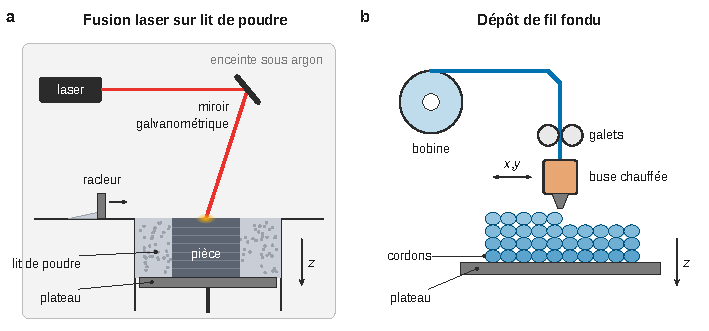
\includegraphics{figures/q2-10-lpbf-fdm.pdf}
\caption*{Figure 5 --- principe de la fusion laser sur lit de poudre (a) et du
dépôt de fil fondu (b)}
\end{figure}

Ces deux procédés ne sont pas des procédés d'assemblage : ils construisent une pièce unique, couche par couche, à partir d'une matière première non mise en forme (poudre ou fil). La fusion n'y soude pas deux pièces existantes, elle lie chaque couche à la précédente.

\begin{piege}

Fusion et soudage ne sont pas synonymes ici : décrire la fusion laser comme le soudage de deux pièces fait perdre tous les points de la question.

\end{piege}

\begin{jury}

Rapport 2026 (p.~3) : « Une part importante des candidat.es a décrit ces procédés comme des procédés d'assemblage de deux pièces par soudure. » Le jury s'en étonne d'autant plus pour le dépôt de fil fondu, procédé des imprimantes 3D grand public. Bilan de Q2.9 à Q2.14 : 8 \% de bonnes réponses.

\end{jury}

\hypertarget{question-2.11}{%
\subsection{Question 2.11}\label{question-2.11}}

\begin{indication}{1}

Qu'y a-t-il sous une surface en porte-à-faux, dans chacun des deux procédés ?

\end{indication}

\begin{indication}{2}

Dans le LPBF, la poudre est présente sous la couche : pourquoi ne suffit-elle pas ? Pensez à la conduction de la chaleur et aux contraintes résiduelles.

\end{indication}

\hypertarget{solution-24}{%
\subsubsection{Solution}\label{solution-24}}

Les deux procédés empilent des couches de bas en haut. Une surface en porte-à-faux, inclinée à moins de 45° environ par rapport au plateau, n'a pas d'appui solide.

\begin{itemize}
\tightlist
\item
  \textbf{FDM} : le cordon déposé dans le vide s'affaisse ; un îlot qui commence en l'air est impossible à fabriquer.
\item
  \textbf{LPBF} : la poudre ne soutient pas efficacement le bain de fusion. Elle conduit mal la chaleur et sa densité apparente est environ moitié de celle du métal. Le bain s'enfonce et surchauffe, la couche se gondole, au risque de heurter le racleur. Les supports ont en outre deux rôles propres au LPBF :

  \begin{itemize}
  \tightlist
  \item
    \textbf{ancrer} la pièce au plateau contre les contraintes résiduelles dues au refroidissement rapide ;
  \item
    \textbf{évacuer la chaleur} vers le plateau.
  \end{itemize}
\end{itemize}

\hypertarget{question-2.12}{%
\subsection{Question 2.12}\label{question-2.12}}

\begin{indication}{1}

Pour chaque critère, demandez-vous ce qu'il fait varier : le temps de fabrication, la quantité de matière, le post-traitement, ou le nombre de pièces par fabrication.

\end{indication}

\begin{indication}{2}

Comparez les deux procédés : dans le LPBF, la poudre est étalée sur tout le plateau à chaque couche ; dans le FDM, la buse ne dépose que là où il y a de la matière.

\end{indication}

\hypertarget{solution-25}{%
\subsubsection{Solution}\label{solution-25}}

\begin{enumerate}
\def\labelenumi{\arabic{enumi}.}
\tightlist
\item
  \textbf{Hauteur}. Le nombre de couches vaut \(h/e\). En LPBF, l'étalement de la poudre sur tout le plateau à chaque couche fixe un temps incompressible par couche, quel que soit le nombre de pièces : la hauteur pilote directement la durée de fabrication et la quantité de poudre engagée. En FDM, le temps dépend surtout du volume déposé, et la hauteur a moins d'effet.
\item
  \textbf{Aire supportée}. Dans les deux procédés, elle détermine la surface dégradée et le temps de retrait des supports. En LPBF, ce retrait est mécanique, long et coûteux, et les surfaces doivent être reprises. En FDM, les supports se détachent ou se dissolvent facilement.
\item
  \textbf{Emprise sur le plateau}. Elle fixe le nombre de pièces par fabrication, donc la répartition des coûts fixes. En LPBF, ces coûts fixes sont élevés (mise sous gaz inerte, dépoudrage, détensionnement, découpe), d'où un grand intérêt à regrouper les pièces. En FDM, le gain est faible car le temps est proportionnel à la matière déposée.
\item
  \textbf{Volume de support}. En LPBF, c'est du métal fondu, coûteux, non récupérable, qui consomme du temps de laser et doit être enlevé mécaniquement. En FDM, c'est un fil bon marché, et l'enjeu est faible.
\end{enumerate}

\begin{piege}

Ces critères s'opposent : coucher la pièce réduit la hauteur mais augmente l'emprise et l'aire supportée. Il faut le noter pour préparer l'arbitrage de la question 2.14.

\end{piege}

\hypertarget{question-2.13}{%
\subsection{Question 2.13}\label{question-2.13}}

\begin{indication}{1}

Cherchez, parmi les comparaisons de Q2.12, le critère qui pèse beaucoup en LPBF métallique et peu en FDM.

\end{indication}

\begin{indication}{2}

Repensez aux rôles des supports en LPBF, établis en Q2.11.

\end{indication}

\hypertarget{solution-26}{%
\subsubsection{Solution}\label{solution-26}}

\textbf{Le critère le plus spécifique au LPBF métallique est le volume de support.} En LPBF, les supports ne servent pas seulement à soutenir les porte-à-faux : ils ancrent la pièce et évacuent la chaleur. Ils sont faits du même métal, soudés à la pièce et au plateau, et ne sont pas recyclables. Ils consomment du temps de laser et exigent un parachèvement coûteux (sciage, électroérosion, usinage). En FDM, le support est un fil bon marché, souvent soluble.

La hauteur est l'autre critère propre au lit de poudre, puisque le temps d'étalement de la poudre est fixe à chaque couche. Elle intervient cependant aussi, dans une moindre mesure, en FDM.

\begin{methode}

Pour une question qui demande le critère « le plus spécifique », annoncez le critère, justifiez-le par une différence de nature entre les deux procédés, puis indiquez pourquoi vous écartez le concurrent le plus sérieux.

\end{methode}

\hypertarget{question-2.14}{%
\subsection{Question 2.14}\label{question-2.14}}

\begin{indication}{1}

Vérifiez d'abord que les quatre couronnes tiennent sur le plateau pour chaque orientation : emprise totale et hauteur.

\end{indication}

\begin{indication}{2}

Repérez une orientation dominée par une autre, puis arbitrez entre les deux qui restent, en restant cohérent avec le critère retenu en Q2.13.

\end{indication}

\hypertarget{solution-27}{%
\subsubsection{Solution}\label{solution-27}}

Bilan pour quatre couronnes :

\begin{longtable}[]{@{}
  >{\raggedright\arraybackslash}p{(\columnwidth - 8\tabcolsep) * \real{0.1643}}
  >{\raggedright\arraybackslash}p{(\columnwidth - 8\tabcolsep) * \real{0.1578}}
  >{\raggedright\arraybackslash}p{(\columnwidth - 8\tabcolsep) * \real{0.1879}}
  >{\raggedright\arraybackslash}p{(\columnwidth - 8\tabcolsep) * \real{0.2232}}
  >{\raggedright\arraybackslash}p{(\columnwidth - 8\tabcolsep) * \real{0.2368}}@{}}
\toprule\noalign{}
\begin{minipage}[b]{\linewidth}\raggedright
\end{minipage} & \begin{minipage}[b]{\linewidth}\raggedright
Hauteur (mm)
\end{minipage} & \begin{minipage}[b]{\linewidth}\raggedright
Emprise × 4 (cm²)
\end{minipage} & \begin{minipage}[b]{\linewidth}\raggedright
Aire supportée × 4 (cm²)
\end{minipage} & \begin{minipage}[b]{\linewidth}\raggedright
Volume de support × 4 (cm³)
\end{minipage} \\
\midrule\noalign{}
\endhead
\bottomrule\noalign{}
\endlastfoot
Orientation 1 & 87,1 & 80,8 & 64,8 & 97,6 \\
Orientation 2 & \textbf{23,7} & 290 & 96,4 & 88,4 \\
Orientation 3 & 88,0 & 159,2 & \textbf{1,2} & \textbf{3,6} \\
\end{longtable}

Le plateau offre 400 cm² et 200 mm de hauteur : les trois orientations sont admissibles. L'orientation 2 occupe toutefois 73 \% du plateau.

\begin{itemize}
\tightlist
\item
  L'orientation 1 est \textbf{dominée} par la 3 : même hauteur, mais 27 fois plus de support.
\item
  L'orientation 2 donne la hauteur minimale (environ 790 couches de 30 µm, contre environ 2 930), au prix de 88 cm³ de supports en titane.
\item
  L'orientation 3 est presque autoportante (0,9 cm³ de support et 0,3 cm² supportés par pièce).
\end{itemize}

\textbf{Orientation retenue : l'orientation 3}, les quatre couronnes disposées en carré (2 × 2) sur le plateau. Elle est cohérente avec le critère de Q2.13 : volume de support divisé par environ 25, presque aucun parachèvement, aucune surface dégradée. Pour une seule fabrication par an, le temps machine supplémentaire est un coût unique et prévisible. Réserve : avec si peu d'appui, l'ancrage contre les contraintes résiduelles est à vérifier, et quelques supports d'ancrage peuvent être nécessaires.

L'orientation 2 se défend si l'on a retenu la hauteur en Q2.13 : les surfaces fonctionnelles étant reprises en usinage, la dégradation des faces supportées pèse moins.

\begin{jury}

Dans une question d'arbitrage, la note dépend surtout de trois éléments : un critère explicite, une comparaison chiffrée et une conclusion cohérente avec ce qu'on a écrit à la question précédente.

\end{jury}

\hypertarget{question-2.15}{%
\subsection{Question 2.15}\label{question-2.15}}

\begin{indication}{1}

Un tour CN « 3 axes » a deux axes linéaires. Quel est le troisième ?

\end{indication}

\begin{indication}{2}

Classez les entités du DR XIII en deux familles : les surfaces de révolution et les trous répartis angulairement. Quels moyens du tour réalisent chacune ?

\end{indication}

\hypertarget{solution-28}{%
\subsubsection{Solution}\label{solution-28}}

\textbf{Cinématique} : axe Z (translation parallèle à la broche), axe X (translation radiale), axe C (rotation de la broche asservie en position, indexable ou interpolable). En tournage, le mouvement de coupe est la rotation de la pièce. En perçage ou en fraisage, c'est la rotation d'un \textbf{outil tournant}, la broche étant bloquée ou indexée.

\textbf{Technologie} :

\begin{itemize}
\tightlist
\item
  mandrin, à mors doux pour une pièce mince ;
\item
  tourelle indexable dont certains emplacements sont \textbf{motorisés} : ils entraînent des outils tournants axiaux (parallèles à Z) et radiaux (parallèles à X), pour les opérations hors de l'axe de rotation de la pièce ;
\item
  interpolation X/Z, cycles de perçage et de taraudage synchronisé, vitesse de coupe constante.
\end{itemize}

\textbf{Justification.}

\begin{itemize}
\tightlist
\item
  Les surfaces internes, les surfaces de guidage des biellettes et les interfaces du roulement sont \textbf{de révolution} : elles se tournent selon X et Z, en \textbf{travail d'enveloppe}. La pointe de l'outil décrit le profil de la surface dans le plan (X, Z) pendant que la pièce tourne, et la forme de l'outil n'est pas recopiée.
\item
  Les \textbf{trous axiaux Ø5} et les \textbf{trous radiaux taraudés M3} des oreilles, répartis à 120°, se réalisent avec des outils tournants et une indexation en C.
\end{itemize}

Tout se fait sur une seule machine, en deux prises de pièce. Les entités liées par une spécification sont usinées dans la même mise en position, ce qui supprime les dispersions dues aux reprises. La denture intérieure n'appartient pas à ces deux phases : elle relève d'une opération spécifique (mortaisage par outil-pignon, brochage).

\begin{piege}

Sur un tour, le troisième axe est l'axe C de la broche, pas un axe linéaire Y.

\end{piege}

\begin{jury}

Rapport 2026 (p.~3) : « cette cinématique est très mal connue des candidat.es, ainsi que la présence d'une tourelle dotée d'emplacements motorisés pour des opérations hors axe de rotation ». La série Q2.15 à Q2.17 est la plus discriminante du sujet : 4 \% de bonnes réponses et 26 \% de copies qui ne la traitent pas.

\end{jury}

\hypertarget{question-2.16}{%
\subsection{Question 2.16}\label{question-2.16}}

\begin{indication}{1}

Rappelez la convention ISO : quel axe est porté par la broche, et dans quel sens est-il orienté ?

\end{indication}

\begin{indication}{2}

Pour chaque outil tournant, l'axe de rotation est imposé par la direction du trou à percer.

\end{indication}

\hypertarget{solution-29}{%
\subsubsection{Solution}\label{solution-29}}

Sur chaque schéma du cahier réponse, on trace :

\begin{itemize}
\tightlist
\item
  \textbf{l'axe du mandrin}, confondu avec l'axe de la couronne ;
\item
  \textbf{Z}, porté par l'axe du mandrin et orienté positivement en s'éloignant du mandrin, c'est-à-dire de la pièce vers l'outil ;
\item
  \textbf{X}, perpendiculaire à Z et orienté positivement en s'éloignant radialement de l'axe ;
\item
  en \textbf{phase 10} : un outil tournant d'axe \textbf{parallèle à Z}, au rayon de 40,4 mm, pour les trous axiaux Ø5, et un outil tournant d'axe \textbf{parallèle à X}, dans le plan radial d'une oreille, pour les trous radiaux M3 ;
\item
  en \textbf{phase 20} : aucun outil tournant.
\end{itemize}

Entre les deux phases, la couronne est retournée. Les axes de la machine restent les mêmes, mais la face de la couronne tournée vers l'outil change.

\begin{piege}

Les trous M3 des oreilles sont radiaux : sur la coupe A-A, ils sont perpendiculaires à l'axe. Leur outil tournant est donc parallèle à X, pas à Z.

\end{piege}

\hypertarget{question-2.17}{%
\subsection{Question 2.17}\label{question-2.17}}

\begin{indication}{1}

Pour chaque opération, donnez quatre informations : le nom de l'outil et sa silhouette orientée, sa trajectoire, ce qui porte le mouvement de coupe, ce qui porte le mouvement d'avance.

\end{indication}

\begin{indication}{2}

Un trou taraudé demande deux opérations, et l'indexation en C entre deux trous fait partie de la trajectoire.

\end{indication}

\hypertarget{solution-30}{%
\subsubsection{Solution}\label{solution-30}}

\textbf{Phase 10 : surfaces internes.} Outil à charioter-dresser intérieur (barre d'alésage), dessiné à l'intérieur de l'alésage, la plaquette tournée vers la paroi. Mouvement de coupe : rotation de la pièce. Avance : translation de l'outil suivant Z puis X. Trajectoire : entrée suivant \(-Z\), chariotage intérieur, dressage des épaulements suivant X, dégagement radial, sortie suivant \(+Z\).

\textbf{Phase 10 : trous axiaux Ø5.} Foret à centrer puis foret Ø5, montés sur un outil tournant axial. Mouvement de coupe : rotation du foret, broche bloquée. Avance : translation de l'outil suivant \(-Z\). Trajectoire : positionnement en X au rayon de 40,4 mm, perçage avec débourrage, retour, indexation de C de 120°, puis deux répétitions.

\textbf{Phase 10 : trous radiaux M3.} Foret Ø2,5 puis taraud M3, montés sur un outil tournant radial. Mouvement de coupe : rotation de l'outil, broche bloquée. Avance suivant \(-X\), synchronisée sur le pas de 0,5 mm par tour pour le taraudage, avec sortie en inversant la rotation. Indexation de C de 120° entre deux trous.

\textbf{Phase 20 : interfaces du roulement.} Outil à charioter-dresser extérieur de finition (plaquette en losange à 35° ou 55°, petit rayon de bec), placé à l'extérieur de la pièce. Son angle de pointe et son angle de direction d'arête (supérieur à 90°) lui permettent de remonter l'épaulement sans que l'arête secondaire talonne. Mouvement de coupe : rotation de la pièce à vitesse de coupe constante. Avance : translation de l'outil suivant Z, puis X. Trajectoire : chariotage de la portée Ø63,5, congé, dressage de l'épaulement, en une seule passe continue. La cylindricité, la position et le battement sont ainsi obtenus dans la même mise en position.

\begin{methode}

En tournage, le mouvement de coupe est porté par la pièce. Avec un outil tournant, il est porté par l'outil et la broche est bloquée. Il faut toujours préciser quel élément tourne.

\end{methode}

\begin{jury}

Rapport 2026 (p.~3) : « La réalisation d'une surface fonctionnelle de révolution par un travail d'enveloppe constitue également une difficulté. » Les trajectoires et les géométries d'outils, sans en apprendre la typologie, « constituent une base fondamentale pour déterminer si une surface est usinable ou non ». Il faut donc dessiner l'outil orienté et vérifier qu'il atteint la surface sans interférer.

\end{jury}

\hypertarget{partie-3-conception-de-la-vertebre}{%
\section{Partie 3 --- Conception de la « VERTEBRE »}\label{partie-3-conception-de-la-vertebre}}

Une seule question, qui vaut à elle seule environ 40 \% du temps. Le rapport 2026 commente séparément chacune des six fonctions, avec des taux de bonnes réponses compris entre 2 \% et 20 \% : chaque fonction est une occasion de se distinguer. Il faut dessiner à l'échelle 2:1 un vérin électrique complet : arbre du réducteur, manchon, vis, écrou, tige, fourreau et chape. Le dessin réunit six fonctions. Pour chacune, on raisonne en trois temps : la \textbf{mise en position} (quelles surfaces, quels ajustements), le \textbf{maintien en position} (souvent imposé par l'énoncé), et la \textbf{faisabilité} (usinage possible, montage, respect des règles de tracé). Le schéma cinématique du DR XIV est le cahier des charges.

\hypertarget{question-3.1}{%
\subsection{Question 3.1}\label{question-3.1}}

\begin{indication}{1}

Commencez par suivre sur le DR XIV le trajet de l'effort axial, de la chape jusqu'au bâti. Où cet effort doit-il être repris, et par où ne doit-il surtout pas passer ?

\end{indication}

\begin{indication}{2}

Le manchon est guidé par un seul roulement, qui se modélise par une rotule, et il est accouplé à l'arbre du réducteur. Quelle liaison l'accouplement doit-il réaliser pour que l'ensemble forme un pivot isostatique ? Regardez aussi attentivement l'arbre du réducteur sur le dessin réponse.

\end{indication}

\begin{indication}{3}

Lisez la référence de la vis IGUS : peut-on usiner une portée lisse au diamètre nominal d'une vis filetée ? Le DR III indique que l'extrémité des vis peut être usinée. Pour la glissière, demandez-vous comment garder une grande distance entre les deux paliers sur toute la course.

\end{indication}

\hypertarget{solution-31}{%
\subsubsection{Solution}\label{solution-31}}

\textbf{Architecture.} Le réducteur entraîne le manchon, guidé en rotation dans la pièce de jonction par un roulement. Le manchon est encastré sur la vis IGUS. L'écrou, encastré dans la tige, ne peut pas tourner, parce que la tige est arrêtée en rotation dans le fourreau. Il se translate donc de 12 mm par tour de vis. La tige porte la chape de liaison. L'effort axial suit le trajet chape, tige, écrou, vis, manchon, roulement, pièce de jonction. \textbf{Il ne doit pas traverser le réducteur.}

\begin{figure}[H]
\centering
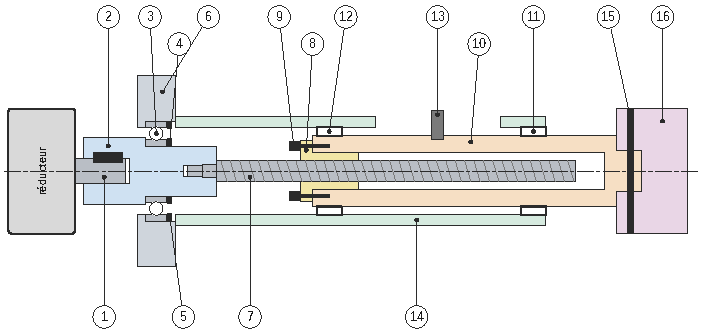
\includegraphics{figures/q3-1-coupe-principe-vertebre.pdf}
\caption*{Figure 6 --- coupe longitudinale de principe de la vertèbre, repères de
la nomenclature (échelle non respectée)}
\end{figure}

\textbf{Nomenclature proposée.}

\begin{longtable}[]{@{}
  >{\raggedright\arraybackslash}p{(\columnwidth - 4\tabcolsep) * \real{0.1422}}
  >{\raggedright\arraybackslash}p{(\columnwidth - 4\tabcolsep) * \real{0.4383}}
  >{\raggedright\arraybackslash}p{(\columnwidth - 4\tabcolsep) * \real{0.3895}}@{}}
\toprule\noalign{}
\begin{minipage}[b]{\linewidth}\raggedright
Repère
\end{minipage} & \begin{minipage}[b]{\linewidth}\raggedright
Désignation
\end{minipage} & \begin{minipage}[b]{\linewidth}\raggedright
Remarque
\end{minipage} \\
\midrule\noalign{}
\endhead
\bottomrule\noalign{}
\endlastfoot
1 & Arbre de sortie du réducteur Ø6, clavette parallèle 2 × 2 & fournis (dessin réponse) \\
2 & Manchon & inox, tourné, rainure mortaisée \\
3 & Roulement rigide à billes inox W 6001 (12 × 28 × 8) & W 61902 (15 × 28 × 7) acceptable \\
4 & Anneau élastique pour arbre & arrêt de la bague intérieure \\
5 & Anneau élastique pour alésage, ou flasque vissé & arrêt de la bague extérieure \\
6 & Pièce de jonction & bâti, bossage pour loger le roulement \\
7 & Vis IGUS DST-LS-10X12-R-AL & extrémité reprise : portée Ø6 h6, filetage M5 \\
8 & Écrou dryspin à collerette & collerette reprise en usinage \\
9 & Trois vis CHC M3 & fixation de l'écrou \\
10 & Tige & tube usiné \\
11 & Palier lisse polymère solidaire du fourreau & emmanché \\
12 & Palier lisse polymère solidaire de la tige & emmanché \\
13 & Doigt d'arrêt en rotation (vis épaulée) & coulisse dans la lumière du fourreau \\
14 & Fourreau & lumière longitudinale fraisée \\
15 & Goupille élastique Ø3 & liaison tige-chape \\
16 & Chape de liaison & fournie, alésage repris \\
\end{longtable}

\textbf{Fonction 1 : accouplement du manchon avec l'arbre du réducteur.}

\begin{itemize}
\tightlist
\item
  \textbf{Centrage} : alésage \textbf{court} Ø6 H7 dans le manchon, sur l'arbre Ø6 g6, sur une longueur d'environ 0,8 d.~On obtient une linéaire annulaire. Avec la rotule du roulement (fonction 2), elle forme un \textbf{pivot isostatique} du manchon : le réducteur n'est pas contraint, même si son arbre et l'alésage de la pièce de jonction sont légèrement désalignés.
\item
  \textbf{Transmission par obstacle} : l'arbre du réducteur porte déjà une \textbf{clavette parallèle}, visible sur le dessin réponse. On réalise dans le moyeu du manchon la \textbf{rainure de clavette correspondante par mortaisage}, un procédé autorisé par l'énoncé. La rainure débouche du côté du réducteur pour permettre le montage par coulissement, avec un jeu au fond de la rainure.
\item
  \textbf{Pas d'arrêt axial} entre l'arbre et le manchon : la clavette parallèle laisse coulisser. C'est le roulement qui positionne le manchon axialement, si bien qu'aucun effort axial ne passe dans les roulements du réducteur.
\item
  \textbf{Tracé} : chanfrein d'entrée, dégagement en fond d'alésage ; la longueur de la rainure couvre celle de la clavette.
\item
  \textbf{Pas de centrage sur le nez du motoréducteur} : le manchon tourne, la face avant et l'épaulement du réducteur sont fixes. Seul l'arbre de sortie centre le manchon.
\end{itemize}

\begin{piege}

Percer l'arbre d'un réducteur du commerce pour y loger une goupille est une mauvaise idée : on modifie un composant acheté alors qu'une clavette est déjà prévue. Un centrage long assorti d'un arrêt axial rendrait de plus la liaison quasi encastrée, et le montage hyperstatique avec la rotule. L'effort axial de la vis passerait alors dans le réducteur.

\end{piege}

\begin{jury}

Rapport 2026 (p.~3), fonction 1 : parmi les erreurs, « de nombreuses solutions non usinables, ainsi que l'utilisation des surfaces à l'avant du moteur réducteur pour centrer le manchon ». Bilan : 14 \% de bonnes réponses. Une rainure de clavette débouchante, réalisable en mortaisage, et un centrage sur l'arbre seul répondent à ces deux reproches.

\end{jury}

\textbf{Fonction 2 : liaison rotule entre le manchon et la pièce de jonction.}

\begin{itemize}
\tightlist
\item
  \textbf{Un seul roulement} rigide à billes en inox, arrêté axialement dans les deux sens, se modélise par une rotule. Choix : \textbf{W 6001 (12 × 28 × 8)}. La portée Ø12 laisse une paroi suffisante autour de l'alésage Ø6 et du taraudage de la vis. La série 60, à billes plus grosses que la série 619, reprend mieux la poussée axiale. Le \textbf{W 61902 (15 × 28 × 7)} convient aussi, avec un manchon plus gros. Le W 608 et le W 626 laisseraient une paroi trop mince autour du Ø6. Le W 61900 (Ø10) en laisserait une juste suffisante.
\item
  \textbf{Ajustements} : la bague intérieure tourne par rapport à la charge, donc elle est \textbf{serrée} sur le manchon (Ø12 k5). La bague extérieure est fixe par rapport à la charge, donc \textbf{glissante} dans la pièce de jonction (Ø28 H7).
\item
  \textbf{Arrêts axiaux} : il en faut quatre, car la vis pousse lorsque le vérin sort et tire lorsqu'il rentre. Avec moins d'arrêts, l'effort axial ne serait repris que dans un sens et la liaison ne serait plus une rotule.

  \begin{itemize}
  \tightlist
  \item
    bague intérieure : épaulement du manchon d'un côté, anneau élastique pour arbre de l'autre ;
  \item
    bague extérieure : épaulement de l'alésage de la pièce de jonction d'un côté, anneau élastique pour alésage ou flasque vissé de l'autre.
  \end{itemize}
\item
  \textbf{Tracé} : la pièce de jonction, dessinée en géométrie simplifiée, est épaissie par un bossage, de sorte que l'alésage Ø28 H7 porte la bague extérieure \textbf{sur toute sa largeur} (8 mm). Hauteurs d'épaulement compatibles avec le démontage, rayons de raccordement inférieurs aux chanfreins des bagues, gorges normalisées pour les anneaux élastiques.
\end{itemize}

\begin{methode}

Pour un roulement modélisé en rotule : la bague tournante par rapport à la charge est montée serrée, la bague fixe est montée glissante, et les arrêts axiaux sont adaptés au sens des efforts. Ici, les efforts changent de sens : il faut les quatre arrêts.

\end{methode}

\begin{piege}

Rapport 2026 (p.~3), fonction 2 : dans une majorité de copies, « les arrêts axiaux ne sont pas en nombre suffisant pour créer une liaison rotule », et souvent « la bague extérieure n'est pas guidée sur toute sa longueur ». Comptez les quatre arrêts sur votre dessin et vérifiez que l'alésage couvre toute la largeur de la bague.

\end{piege}

\textbf{Fonction 3 : encastrement du manchon et de la vis.}

\begin{itemize}
\tightlist
\item
  La référence « 10X12 » indique un diamètre nominal de 10 mm, c'est-à-dire le diamètre à la crête du filet roulé, et un pas de 12 mm. \textbf{Aucune portée lisse Ø10 ne peut être usinée dans la vis.} IGUS autorise l'usinage des extrémités (DR III) : on reprend le bout de la vis en tournage pour obtenir une \textbf{portée Ø6 h6}, inférieure au diamètre du noyau, puis une \textbf{face dressée} qui sert d'épaulement, et enfin un \textbf{filetage M5}.
\item
  \textbf{Centrage} : la portée Ø6 h6 s'engage dans un alésage Ø6 H7 du manchon.
\item
  \textbf{Mise en position axiale} : appui plan de l'épaulement de la vis contre la face frontale du manchon.
\item
  \textbf{Immobilisation par vissage} : le filetage M5 se visse dans un taraudage du manchon, et le serrage plaque l'épaulement. Comme le couple change de sens selon le sens de déplacement, on freine par un frein-filet, ou on ajoute une goupille de sécurité.
\item
  \textbf{Tracé} : gorge de dégagement entre la portée et le filet, chanfreins, fond de taraudage dégagé.
\item
  \textbf{Montage} : aucune vis rapportée. La vis se visse directement dans le manchon avant l'engagement sur l'arbre du réducteur, le manchon étant tenu par deux méplats. L'ensemble reste compact et démontable.
\end{itemize}

\begin{piege}

Le diamètre nominal d'une vis filetée est celui des crêtes du filet. Une portée de centrage s'usine toujours à un diamètre inférieur au noyau.

\end{piege}

\begin{jury}

Rapport 2026 (p.~3), fonction 3 : dans la solution industrielle, la vis possède « une deuxième partie filetée et un centrage » qui se vissent dans le manchon. Les copies ont surtout ajouté des vis encombrantes, et « L'accessibilité aux vis et la facilité de montage de l'ensemble ont souvent fait défaut. » Bilan : 5 \% de bonnes réponses.

\end{jury}

\textbf{Fonction 4 : encastrement de l'écrou et de la tige.}

\begin{itemize}
\tightlist
\item
  On choisit l'\textbf{écrou dryspin à collerette} du DR III, que l'on peut reprendre en usinage.
\item
  \textbf{Centrage} : le corps de l'écrou s'engage dans un alésage H7 usiné à l'extrémité de la tige (ajustement glissant juste).
\item
  \textbf{Appui} : la face de la collerette vient en appui plan sur la face d'extrémité de la tige.
\item
  \textbf{Immobilisation} : \textbf{trois vis CHC M3} à 120°, passant dans les trous de la collerette et vissées dans des taraudages de la tige. Le couple et l'effort axial sont transmis par l'appui plan, par l'adhérence sous serrage et par les vis.
\item
  L'écrou est une pièce d'usure : l'assemblage doit rester démontable, ce qui exclut le collage et le frettage.
\item
  \textbf{Montabilité et usinage} : l'écrou est fixé à la tige avant l'introduction de la vis et avant l'engagement de la tige dans le fourreau. Les têtes de vis restent alors accessibles par l'extrémité de la tige. L'alésage, la face d'appui et les taraudages débouchent tous sur cette extrémité et se réalisent en tournage et perçage, sans rainure ni forme non débouchante. La collerette est reprise au diamètre de la tige, pour une géométrie compacte.
\end{itemize}

\begin{piege}

Une rainure de clavette non débouchante dans un alésage ne se réalise ni en mortaisage ni en brochage. Avant de dessiner une forme, demandez-vous avec quel outil et par quel côté elle sera usinée, et dans quel ordre les pièces seront montées.

\end{piege}

\begin{jury}

Rapport 2026 (p.~4) : c'est la fonction la moins réussie du sujet (2 \% de bonnes réponses). Les deux écueils sont « la montabilité et la réalisation des surfaces fonctionnelles, notamment dans le cas de rainures de clavette non débouchantes ». Le jury note aussi que les formes d'écrous proposées ont peu inspiré et que les solutions correctes étaient souvent très massives.

\end{jury}

\textbf{Fonction 5 : glissière entre la tige et le fourreau.}

\begin{itemize}
\tightlist
\item
  \textbf{Guidage} par une \textbf{paire de paliers lisses} en polymère autolubrifiant, sans graisse et compatibles avec l'eau potable :

  \begin{itemize}
  \tightlist
  \item
    le premier palier est \textbf{solidaire du fourreau}, emmanché à son extrémité, et guide le diamètre extérieur de la tige ;
  \item
    le second palier est \textbf{solidaire de la tige}, emmanché à son extrémité intérieure, et glisse dans l'alésage du fourreau.
  \end{itemize}

  Dans ce montage télescopique, la distance entre les deux paliers reste grande pendant toute la course, ce qui évite l'arc-boutement (longueur guidée supérieure à 1,5 fois le diamètre). Ajustements : paliers emmanchés serrés dans leurs logements, jeu de glissement H8/f7, surfaces de glissement rectifiées.
\item
  \textbf{Arrêt en rotation par obstacle} : un \textbf{doigt} (vis épaulée) fixé sur la tige coulisse dans une \textbf{lumière longitudinale fraisée} dans le fourreau. La longueur de la lumière vaut la course plus la largeur du doigt. Variante : rainure intérieure mortaisée et clavette vissée sur la tige. Cet arrêt reprend le couple que la vis transmet à l'écrou.
\end{itemize}

\begin{methode}

Une glissière de grande course se réalise en général par deux paliers éloignés, dont l'un se déplace avec la pièce mobile, et un arrêt en rotation séparé. Les deux fonctions sont bien distinctes.

\end{methode}

\textbf{Fonction 6 : encastrement de la tige et de la chape de liaison.}

\begin{itemize}
\tightlist
\item
  \textbf{Mise en position} : appui plan prépondérant (épaulement de la tige contre la face de la chape) et centrage court (Ø H7/g6). L'appui plan impose l'orientation de la chape, et le centrage court sa position radiale, sans hyperstatisme. \textbf{Un seul appui axial} : le fond de l'alésage de la chape est dégagé, avec du jeu devant l'extrémité de la tige.
\item
  \textbf{Immobilisation par goupille} : une \textbf{goupille élastique Ø3} traverse la chape et la tige perpendiculairement à l'axe, dans un perçage réalisé au montage. Elle supprime la rotation restante et transmet l'effort de traction en double cisaillement. En compression, l'effort passe par l'appui plan.
\item
  \textbf{Position de la goupille} : la vis pénètre dans la tige sur toute la course. La goupille est donc placée \textbf{au-delà de l'extrémité de la vis en position rentrée}, avec une marge de sécurité, pour ne jamais croiser la vis.
\item
  \textbf{Tracé} : distance suffisante entre le perçage et l'extrémité de la tige pour éviter l'arrachement, chanfreins d'entrée.
\end{itemize}

\begin{piege}

Rapport 2026 (p.~4), fonction 6 : « Les goupilles ont souvent traversé la vis et les mises en position axiale comportaient trop d'appuis. » Tracez la vis dans sa position la plus engagée avant de placer la goupille, et ne gardez qu'une surface d'appui axial.

\end{piege}

\textbf{Récapitulatif.}

\begin{longtable}[]{@{}
  >{\raggedright\arraybackslash}p{(\columnwidth - 4\tabcolsep) * \real{0.2695}}
  >{\raggedright\arraybackslash}p{(\columnwidth - 4\tabcolsep) * \real{0.3431}}
  >{\raggedright\arraybackslash}p{(\columnwidth - 4\tabcolsep) * \real{0.3574}}@{}}
\toprule\noalign{}
\begin{minipage}[b]{\linewidth}\raggedright
Fonction
\end{minipage} & \begin{minipage}[b]{\linewidth}\raggedright
Mise en position
\end{minipage} & \begin{minipage}[b]{\linewidth}\raggedright
Maintien en position
\end{minipage} \\
\midrule\noalign{}
\endhead
\bottomrule\noalign{}
\endlastfoot
Arbre du réducteur et manchon & centrage court Ø6 H7/g6 & clavette fournie, rainure mortaisée dans le manchon \\
Manchon et pièce de jonction & 1 roulement W 6001, Ø12 k5 et Ø28 H7 & 4 arrêts axiaux \\
Manchon et vis & centrage Ø6 H7/h6 et appui plan & filetage M5 et frein-filet \\
Écrou et tige & centrage H7 et appui plan sur la collerette & 3 vis CHC M3 \\
Tige et fourreau & 2 paliers lisses (fourreau, tige) & doigt dans une lumière \\
Tige et chape & appui plan (seul appui axial) et centrage court & goupille élastique Ø3, hors de la course de la vis \\
\end{longtable}

\begin{jury}

Rapport 2026 (pp.~3-4) : chaque fonction est évaluée séparément. Taux de bonnes réponses : accouplement 14 \%, rotule 19 \%, encastrement manchon-vis 5 \%, glissière 20 \%, encastrement écrou-tige 2 \%, goupille tige-chape 5 \%. Les deux dernières fonctions ont été moins abordées, sans doute du fait de leur position en fin de sujet : 20 \% et 25 \% de copies ne les traitent pas. Il vaut mieux traiter les six fonctions, même sommairement, qu'en détailler trois, en vérifiant pour chacune l'usinage et le montage.

\end{jury}

\hypertarget{bilan}{%
\section{Bilan}\label{bilan}}

\textbf{Méthodes à retenir.}

\begin{itemize}
\tightlist
\item
  \textbf{Codeurs incrémentaux} : la quadrature multiplie la résolution par 4 et donne le sens de rotation ; l'index sert de référence une fois par tour. Pour calculer une résolution, on remonte toute la chaîne de transmission : codeur, réducteur, vis.
\item
  \textbf{Diagramme d'états} : la durée d'un cycle se calcule sur le chemin critique. Les branches parallèles se combinent par leur maximum.
\item
  \textbf{Fermeture géométrique} : pour savoir si un mécanisme peut bouger, il faut raisonner en déplacements finis. Une étude en vitesses dans une configuration singulière peut tromper.
\item
  \textbf{Hyperstatisme} : \(m - h = I_c - E_c\). La fermeture cinématique indique \textbf{quelles} inconnues sont hyperstatiques, ce qui permet de choisir la liaison à modifier (ici, une linéaire rectiligne).
\item
  \textbf{Trains d'engrenages à axes fixes} : un engrènement extérieur change le signe, un engrènement intérieur le conserve, et une roue intermédiaire inverse le sens sans changer le module du rapport.
\item
  \textbf{Loi entrée-sortie} : on la lit sur la courbe, et on teste l'interprétation de l'angle avec une durée donnée dans le dossier.
\item
  \textbf{Fiches GPS} : type, élément tolérancé, références, zone, contraintes. La direction de la flèche distingue un battement radial d'un battement axial.
\item
  \textbf{Indice de performance} : on élimine la variable géométrique libre ; dans le diagramme log-log, l'indice devient une droite de pente \(1/n\) (ici 3/2).
\item
  \textbf{Petite série} : l'amortissement de l'outillage écarte les procédés à moule ou à matrice.
\item
  \textbf{Fabrication additive} : supports, hauteur, emprise et aire supportée s'opposent. Le choix d'orientation doit découler du critère jugé prioritaire.
\item
  \textbf{Tour 3 axes} : axes X, Z et C, outils tournants, et regroupement dans une même prise de pièce des surfaces liées par des spécifications.
\item
  \textbf{Conception} : distinguer la mise en position du maintien en position, s'assurer qu'une rotule et un accouplement forment un pivot isostatique, et faire reprendre l'effort axial au plus près, sans le faire passer par le réducteur.
\end{itemize}

\textbf{Ce que retient le rapport 2026.} Les reproches portent moins sur les calculs que sur la lecture des documents et la culture technologique : capteur absolu ou relatif, vérification d'une performance par un modèle au lieu de la recopier, notion de taille entre deux points, lecture d'un diagramme d'Ashby, principe des procédés additifs, cinématique d'un tour à axe C, montabilité des solutions dessinées. Le jury rappelle enfin que « Les ordres de grandeur de longueur, de masse, de force ou de puissance sont à connaître pour éviter des résultats aberrants. »

\textbf{Prérequis à revoir} : la norme ISO GPS (taille entre deux points, principe d'indépendance, battements), le tableau des liaisons usuelles et leurs degrés de liberté, les ajustements de roulements, les procédés de fabrication additive et les conventions d'axes des machines-outils.

\textbf{Questions classiques transposables} : la résolution d'un codeur ramenée à un déplacement linéaire ; la durée d'un cycle donné par un diagramme d'états ; la liaison à modifier pour rendre un mécanisme isostatique ; un rapport de train à axes fixes avec dentures intérieures ; une fiche GPS ; un indice d'Ashby pour une poutre en flexion (\(n = 2/3\)) ; l'orientation d'une pièce en fabrication additive ; la conception d'un vérin électrique (vis, écrou, glissière avec arrêt en rotation, roulement modélisé en rotule).

\end{document}
